\documentclass[conference]{IEEEtran}
\IEEEoverridecommandlockouts
\usepackage{cite}
\usepackage{amsmath,amssymb,amsfonts}
\usepackage{graphicx}
\usepackage{textcomp}
\usepackage{xcolor}
\usepackage{booktabs}
\usepackage{multirow}
\usepackage{tikz}
\usetikzlibrary{positioning,arrows.meta,fit,shapes.geometric,calc}
\usepackage{hyperref}
\usepackage{url}
\graphicspath{{figures/}}

\tikzset{
  blk/.style={draw, rounded corners=2pt, minimum height=6mm, minimum width=9mm, font=\scriptsize, align=center, fill=blue!6},
  lat/.style={draw, rounded corners=2pt, minimum height=6mm, minimum width=7mm, font=\scriptsize, align=center, fill=orange!20},
  op/.style={draw, circle, inner sep=1pt, font=\scriptsize},
  arr/.style={-{Latex[length=1.6mm]}, thick},
}

% generated by scripts/make_report_assets.py
\newcommand{\AUTHORNAME}{Muhammad Ibrahim Malik (23i-0694)}
\newcommand{\AUTHORAFFIL}{Department of Computer Science, FAST-NUCES Islamabad, Pakistan\\Course instructor: Dr.~Akhtar Jamil}
\newcommand{\VIDEOURL}{https://youtube.com/}
\newcommand{\WANDBURL}{https://wandb.ai/m-ibrahim-malik-national-university-of-computer-and-eme/genai-a1}
\newcommand{\NTRAIN}{2944}
\newcommand{\NVAL}{736}
\newcommand{\NTEST}{3669}
\newcommand{\NTESTENTRIES}{36690}
\newcommand{\NTRAINVAL}{3680}
\newcommand{\TONETRIALS}{14}
\newcommand{\TONEPRUNED}{8}
\newcommand{\TONEBEST}{13}
\newcommand{\TONEBESTVAL}{0.6685}
\newcommand{\TONELR}{7.3e-04}
\newcommand{\TONEBS}{16}
\newcommand{\TONELATCH}{16}
\newcommand{\TONEBASE}{64}
\newcommand{\TONEDROP}{0.012}
\newcommand{\TONEALPHA}{0.557}
\newcommand{\TONELATDIM}{4{,}096}
\newcommand{\TONECOMPRESS}{12}
\newcommand{\TONEEPOCHS}{45}
\newcommand{\TONETRIALEP}{6}
\newcommand{\CLSTRIALS}{10}
\newcommand{\CLSBESTPARAMS}{lr=7.6e-04, batch=32, channels=large, dropout=0.136, wd=0.002}
\newcommand{\SPTRIALS}{8}
\newcommand{\SPBESTPARAMS}{lr=2.4e-04, batch=16, $c_z$=32, $b$=48, $\alpha$=0.769}
\newcommand{\SPEPOCHS}{35}
\newcommand{\MOETRIALS}{8}
\newcommand{\MOEBESTPARAMS}{$\lambda_1$=0.509, lr=2.7e-04, $\tau$=1.749, $\lambda_c$=0.023, $\lambda_b$=0.002}
\newcommand{\MOECOLLAPSED}{0}
\newcommand{\MOEWARM}{2}
\newcommand{\MOEEPOCHS}{12}
\newcommand{\TONEPSNRCORR}{25.99}
\newcommand{\TONESSIMCORR}{0.817}
\newcommand{\PREDPSNRCORR}{26.12}
\newcommand{\PREDSSIMCORR}{0.808}
\newcommand{\ORACLEPSNRCORR}{26.11}
\newcommand{\ORACLESSIMCORR}{0.808}
\newcommand{\MOEPSNRCORR}{26.46}
\newcommand{\MOESSIMCORR}{0.838}
\newcommand{\INPUTPSNRCORR}{19.27}
\newcommand{\INPUTSSIMCORR}{0.633}
\newcommand{\ONNXMAXDIFF}{2.0e-06}
\newcommand{\FSTRAIN}{899}
\newcommand{\FSVAL}{159}
\newcommand{\FSTEST}{1046}
\newcommand{\FSTRAINFULL}{1058}
\newcommand{\FSVALSTYLES}{54/52/53}
\newcommand{\FSTRIALS}{12}
\newcommand{\FSBESTPARAMS}{lr$_G$=4.0e-04, lr$_D$=4.5e-05, batch=8, $b$=48, dropout=0.465, $d$=16, $\lambda_{L1}$=111.071}
\newcommand{\FSEPOCHS}{200}
\newcommand{\FSTRIALEP}{30}
   % generated numbers (\newcommand definitions)

\begin{document}

\title{From Universal Denoising to Soft Mixture-of-Experts Restoration and Style-Conditioned Face-to-Sketch Synthesis: Design, Optimisation and Deployment of Four Generative Systems}

\author{\IEEEauthorblockN{\AUTHORNAME}
\IEEEauthorblockA{\AUTHORAFFIL\\
Generative AI --- Assignment 1\\
Code: \url{https://github.com/ibrahimmlk/Generative-AI-Assignment-1}\\
Demo video: \url{\VIDEOURL}}}

\maketitle

\begin{abstract}
We design, train, evaluate and deploy four related generative systems. Tasks~1--3 restore $128\times128$ Oxford-IIIT Pet images corrupted at run time by salt-and-pepper noise, Gaussian blur or rectangular occlusion: (1) a single universal convolutional denoising autoencoder (DAE) with a genuine latent bottleneck, (2) a hard-routed system in which a CNN corruption classifier selects one of three specialist DAEs, and (3) a differentiable soft mixture-of-experts (MoE) whose gate is initialised from the classifier and trained jointly with the experts under reconstruction, SSIM, cross-entropy and routing-balance losses. Task~4 is a style-conditioned pix2pix GAN that converts FS2K face photographs into sketches in one of three styles using a learned style embedding injected into both generator and discriminator. Every model was tuned with Optuna (TPE sampler, median pruning, routing-collapse pruning for the MoE), tracked with Weights~\&~Biases, exported to ONNX (max.\ deviation from PyTorch $\le\ONNXMAXDIFF$) and served through a React/Tailwind front end and FastAPI back end started by a single Docker Compose command. On the official test set the MoE reaches \MOEPSNRCORR\,dB / \MOESSIMCORR{} SSIM averaged over all corrupted inputs, compared with \TONEPSNRCORR\,dB / \TONESSIMCORR{} for the universal DAE and \PREDPSNRCORR\,dB / \PREDSSIMCORR{} for predicted hard routing.
\end{abstract}

\begin{IEEEkeywords}
denoising autoencoder, image restoration, mixture of experts, conditional GAN, pix2pix, Optuna, ONNX
\end{IEEEkeywords}

%=====================================================================
\section{Introduction}
Real images are degraded in many different ways, and a practical restoration system rarely knows which degradation it faces. Three design philosophies exist: a single \emph{universal} model that must internalise every degradation, a \emph{hard-routed} pipeline that first recognises the degradation and then calls a specialist, and a \emph{soft} mixture that blends specialists with input-dependent weights. We implement all three on the same data, the same corruption definitions and the same evaluation protocol, so their behaviour can be compared directly, and complement them with a paired image-to-image GAN for face-to-sketch synthesis. The contributions of this report are: (i) a reproducible runtime corruption pipeline with deterministic validation/test manifests; (ii) a controlled comparison of universal, hard-routed and soft-routed restoration including oracle versus predicted routing and an analysis of routing behaviour; (iii) a style-conditioned pix2pix model; and (iv) a containerised application that exposes all four models through ONNX Runtime.

%=====================================================================
\section{Related Work}
\textbf{Denoising autoencoders.} Vincent \emph{et al.}~\cite{vincent2008} showed that reconstructing clean inputs from corrupted ones forces an autoencoder to learn robust features; convolutional variants such as DnCNN~\cite{zhang2017dncnn} and RED-Net~\cite{mao2016red} became strong restoration baselines. RED-Net and U-Net~\cite{ronneberger2015} rely on skip connections; we deliberately avoid them in Tasks 1--3 because unrestricted skips let the network copy the input around the bottleneck, which the assignment rules out and which would also copy impulse noise to the output.

\textbf{Loss functions.} Zhao \emph{et al.}~\cite{zhao2017loss} showed that $\ell_2$ training correlates poorly with perceived quality and that a mix of $\ell_1$ and (MS-)SSIM~\cite{wang2004ssim} gives sharper, more structurally faithful restorations. This motivates our $\alpha\mathcal{L}_{L1}+(1-\alpha)(1-\text{SSIM})$ objective with $\alpha$ tuned by Optuna.

\textbf{All-in-one restoration.} AirNet~\cite{li2022airnet} and PromptIR~\cite{potlapalli2023promptir} restore several unknown degradations with one network by learning degradation representations, which is the universal setting of Task~1; our Task~2/3 systems make the degradation representation explicit through a classifier/gate.

\textbf{Mixture of experts.} Jacobs \emph{et al.}~\cite{jacobs1991} introduced gated expert mixtures; Shazeer \emph{et al.}~\cite{shazeer2017} and the Switch Transformer~\cite{fedus2021switch} showed that without an auxiliary load-balancing term the gate collapses onto a few experts. Our routing-balance regulariser follows this line; temperature-scaled softmax gating~\cite{hinton2015distill} controls sharpness.

\textbf{Conditional GANs.} GANs~\cite{goodfellow2014}, conditional GANs~\cite{mirza2014} and pix2pix~\cite{isola2017} (U-Net generator, PatchGAN discriminator, $\lambda_{L1}=100$) form the basis of Task~4. FS2K~\cite{fan2022fs2k} is a recent facial-sketch benchmark with three sketch styles. Categorical conditioning through learned embeddings follows~\cite{mirza2014,odena2017acgan}.

\textbf{Hyper-parameter optimisation and deployment.} Optuna~\cite{akiba2019optuna} provides define-by-run search with the TPE sampler~\cite{bergstra2011tpe} and median pruning. ONNX~\cite{onnx} and ONNX Runtime decouple training from serving.

%=====================================================================
\section{Data and Runtime Corruption Pipeline}
\subsection{Datasets and splits}
Oxford-IIIT Pet~\cite{parkhi2012pets} provides \NTRAINVAL{} official train+val and \NTEST{} official test images (37 breeds; labels unused). The train+val set was split 80/20 with seed 42 into \NTRAIN{} training and \NVAL{} validation images; the same split is used for Tasks 1--3 and the test set was only touched by the final evaluation script. All images are converted to RGB and resized to $128\times128$ with area interpolation and cached as a compressed array.

\subsection{Corruptions}
Table~\ref{tab:corr} lists the corruption definitions. During training, \texttt{RuntimeCorruptionDataset.\_\_getitem\_\_} draws a new condition and a new severity every time an image is loaded, from fresh OS entropy (so workers and epochs never repeat). The condition is chosen with equal probability; for the classifier and the MoE a \texttt{BalancedBatchSampler} additionally forces exactly $B/4$ samples of each class per batch. Salt-and-pepper replaces the selected pixels (all three channels) with black or white with probability $\tfrac12$ each. Occlusion masks are placed without overlap, which makes the joint coverage equal to the sum of the rectangle areas, and a placement is accepted only if the coverage is within $\pm1$\,\% of the sampled target, so the 10--35\,\% constraint is satisfied exactly (measured training range: 10.9--34.2\,\%).

\begin{table}[t]
\centering
\caption{Corruption configuration}
\label{tab:corr}
\resizebox{\columnwidth}{!}{%
\begin{tabular}{lll}
\toprule
Condition & Training (random per load) & Test: low / medium / high \\
\midrule
Clean & identity & identity \\
Salt \& pepper & $p\sim\mathcal{U}(0.02,0.15)$, black/white 50:50 & $p=0.03 / 0.08 / 0.15$ \\
Gaussian blur & $k\in\{3,5,7\}$, $\sigma\sim\mathcal{U}(0.5,2.5)$ & $(3,0.7) / (5,1.5) / (7,2.5)$ \\
Occlusion & 1--3 black boxes, 10--35\,\% area & 1/2/3 boxes, 10/20/35\,\% \\
\bottomrule
\end{tabular}}
\end{table}

\subsection{Deterministic manifests}
Validation and test corruptions are generated once by \texttt{build\_manifests} and stored as JSON with the condition, severity bucket, parameters (probability, kernel/$\sigma$, rectangle coordinates, coverage) and the per-image seed that regenerates the salt-and-pepper mask. The validation manifest assigns one balanced condition per image with severities drawn from the training ranges; the test manifest contains, for each of the \NTEST{} test images, the clean image plus the three corruptions at the three fixed severities (10 entries per image, \NTESTENTRIES{} in total).

%=====================================================================
\section{Task 1: Universal Denoising Autoencoder}
\subsection{Architecture}
The encoder (Fig.~\ref{fig:ae}) is a stem of two $3\times3$ conv--BN--LeakyReLU layers followed by three stride-2 stages, so the spatial size goes $128\to64\to32\to16$ while channels grow $b\to2b\to4b\to8b$. A $1\times1$ convolution then compresses the $8b$ feature maps into a latent tensor of $16\times16\times c_z$; this is the only path to the decoder (no skip connections). The decoder mirrors the encoder using bilinear upsampling followed by convolution, which avoids the checkerboard artefacts of transposed convolutions~\cite{odena2016deconv}, and ends with a sigmoid. With the selected $c_z=\TONELATCH$ the latent has \TONELATDIM{} values, a \TONECOMPRESS$\times$ reduction relative to the $49{,}152$-dimensional input, so the network is forced to learn a compressed representation rather than an identity map. Spatial dropout before and after the bottleneck regularises the latent.

We considered a fully-connected latent vector but rejected it: in preliminary reasoning and smoke tests it discards the spatial layout and produces blurry reconstructions even of clean images, while a narrow convolutional bottleneck retains locality at a comparable compression ratio. We also considered limited skip connections; we did not use them because even a single high-resolution skip lets impulse noise and occluder edges pass straight to the output, defeating the restoration objective.

\begin{figure}[t]
\centering
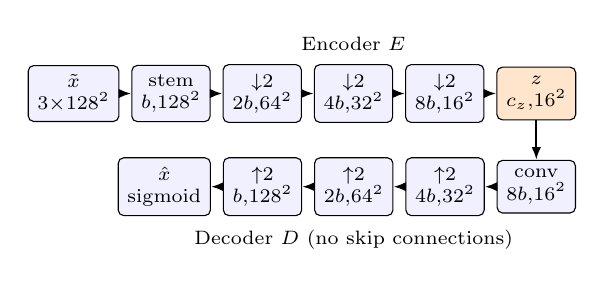
\begin{tikzpicture}[node distance=1.5mm]
\node[blk] (in) {$\tilde{x}$\\3$\times$128$^2$};
\node[blk, right=of in] (e0) {stem\\$b$,128$^2$};
\node[blk, right=of e0] (e1) {$\downarrow$2\\$2b$,64$^2$};
\node[blk, right=of e1] (e2) {$\downarrow$2\\$4b$,32$^2$};
\node[blk, right=of e2] (e3) {$\downarrow$2\\$8b$,16$^2$};
\node[lat, right=of e3] (z) {$z$\\$c_z$,16$^2$};
\node[blk, below=5mm of z] (d0) {conv\\$8b$,16$^2$};
\node[blk, left=of d0] (d1) {$\uparrow$2\\$4b$,32$^2$};
\node[blk, left=of d1] (d2) {$\uparrow$2\\$2b$,64$^2$};
\node[blk, left=of d2] (d3) {$\uparrow$2\\$b$,128$^2$};
\node[blk, left=of d3] (out) {$\hat{x}$\\sigmoid};
\foreach \a/\b in {in/e0,e0/e1,e1/e2,e2/e3,e3/z,z/d0,d0/d1,d1/d2,d2/d3,d3/out} \draw[arr] (\a) -- (\b);
\node[font=\scriptsize, above=0.5mm of e2] {Encoder $E$};
\node[font=\scriptsize, below=0.5mm of d2] {Decoder $D$ (no skip connections)};
\end{tikzpicture}
\caption{Universal DAE $\hat{x}=D(E(\tilde{x}))$. Each block is two $3\times3$ conv--BN--LeakyReLU layers; $\downarrow$2 = stride-2 conv, $\uparrow$2 = bilinear upsampling. The orange $1\times1$-conv latent is the bottleneck. The same architecture is reused for the three Task-2 specialists.}
\label{fig:ae}
\end{figure}

\subsection{Loss and training}
The model minimises $\mathcal{L}_{UDAE}=\alpha\mathcal{L}_{L1}(x,\hat{x})+(1-\alpha)(1-\text{SSIM}(x,\hat{x}))$ with an $11\times11$ Gaussian-window SSIM ($\sigma=1.5$) implemented in PyTorch and computed in FP32 even under mixed precision. We use AdamW (weight decay $10^{-5}$), cosine learning-rate decay, automatic mixed precision and horizontal-flip augmentation of the clean image before corruption, and keep the weights of the epoch with the best validation objective
\begin{equation}
S=\tfrac12\,\text{SSIM}+\tfrac12\,\min(\text{PSNR},40)/40,
\end{equation}
which combines reconstruction quality (PSNR) and structure (SSIM) on comparable $[0,1]$ scales.

\subsection{Optuna study}
Table~\ref{tab:optuna1} gives the search space. The TPE sampler (seed 42) proposed \TONETRIALS{} trials of \TONETRIALEP{} epochs each; a median pruner (3 start-up trials, 1 warm-up epoch) stopped \TONEPRUNED{} unpromising trials. The best trial (\#\TONEBEST, $S=\TONEBESTVAL$) was retrained for \TONEEPOCHS{} epochs. Fig.~\ref{fig:optuna} shows the optimisation histories and parameter importances.

\begin{table}[t]
\centering
\caption{Task 1 Optuna search space and selected configuration}
\label{tab:optuna1}
\begin{tabular}{lll}
\toprule
Hyper-parameter & Range & Selected \\
\midrule
Learning rate & $[10^{-4},3\cdot10^{-3}]$ log & \TONELR \\
Batch size & \{16, 32, 64\} & \TONEBS \\
Bottleneck channels $c_z$ & \{8, 16, 32\} & \TONELATCH \\
Base channels $b$ & \{32, 48, 64\} & \TONEBASE \\
Dropout & $[0, 0.3]$ & \TONEDROP \\
Loss weight $\alpha$ & $[0.5, 0.95]$ & \TONEALPHA \\
\bottomrule
\end{tabular}
\end{table}

\subsection{Results}
Tables~\ref{tab:psnr_type}--\ref{tab:ssim_sev} report PSNR and SSIM on the full official test set (\NTEST{} images $\times$ 10 conditions) for all restoration systems; the ``Input'' column is the corrupted image itself, i.e.\ the no-restoration baseline. Fig.~\ref{fig:t1ex} shows twelve representative examples and Fig.~\ref{fig:t1fail} four failure cases; Fig.~\ref{fig:curves} shows the training curves.

\begin{table}[t]
\centering
\caption{Test PSNR (dB) by input condition}
\label{tab:psnr_type}
\resizebox{\columnwidth}{!}{%
\begin{tabular}{lccccc}
\toprule
Condition & Input & T1 & T2-Oracle & T2-Pred & T3-MoE \\
\midrule
clean & $\infty$ & 12.13 & $\infty$ & 12.11 & 14.65 \\
salt-pepper & 16.55 & 12.13 & 12.11 & 12.11 & \textbf{14.21} \\
blur & 47.29 & 12.13 & 12.11 & 12.11 & \textbf{14.61} \\
occlusion & 12.32 & 12.13 & 12.11 & 12.11 & \textbf{13.62} \\
\bottomrule
\end{tabular}}
\end{table}

\begin{table}[t]
\centering
\caption{Test SSIM by input condition}
\label{tab:ssim_type}
\resizebox{\columnwidth}{!}{%
\begin{tabular}{lccccc}
\toprule
Condition & Input & T1 & T2-Oracle & T2-Pred & T3-MoE \\
\midrule
clean & \textbf{1.000} & 0.323 & \textbf{1.000} & 0.320 & 0.602 \\
salt-pepper & 0.325 & 0.323 & 0.320 & 0.320 & \textbf{0.403} \\
blur & 0.997 & 0.323 & 0.320 & 0.320 & \textbf{0.596} \\
occlusion & 0.697 & 0.323 & 0.320 & 0.320 & \textbf{0.503} \\
\bottomrule
\end{tabular}}
\end{table}

\begin{table}[t]
\centering
\caption{Test PSNR (dB) by corruption and severity}
\label{tab:psnr_sev}
\resizebox{\columnwidth}{!}{%
\begin{tabular}{lccccc}
\toprule
Condition & Input & T1 & T2-Oracle & T2-Pred & T3-MoE \\
\midrule
blur / high & 40.29 & 12.13 & 12.11 & 12.11 & \textbf{14.57} \\
blur / low & 55.15 & 12.13 & 12.11 & 12.11 & \textbf{14.64} \\
blur / medium & 46.43 & 12.13 & 12.11 & 12.11 & \textbf{14.61} \\
clean / none & $\infty$ & 12.13 & $\infty$ & 12.11 & 14.65 \\
occlusion / high & 9.66 & 12.12 & 12.11 & 12.11 & \textbf{13.06} \\
occlusion / low & 15.35 & 12.13 & 12.11 & 12.11 & \textbf{14.17} \\
occlusion / medium & 11.95 & 12.13 & 12.11 & 12.11 & \textbf{13.61} \\
salt-pepper / high & 13.29 & 12.13 & 12.11 & 12.11 & \textbf{13.90} \\
salt-pepper / low & 20.28 & 12.13 & 12.11 & 12.11 & \textbf{14.49} \\
salt-pepper / medium & 16.06 & 12.13 & 12.11 & 12.11 & \textbf{14.24} \\
\bottomrule
\end{tabular}}
\end{table}

\begin{table}[t]
\centering
\caption{Test SSIM by corruption and severity}
\label{tab:ssim_sev}
\resizebox{\columnwidth}{!}{%
\begin{tabular}{lccccc}
\toprule
Condition & Input & T1 & T2-Oracle & T2-Pred & T3-MoE \\
\midrule
blur / high & 0.994 & 0.323 & 0.320 & 0.320 & \textbf{0.590} \\
blur / low & 0.999 & 0.323 & 0.320 & 0.320 & \textbf{0.601} \\
blur / medium & 0.998 & 0.323 & 0.320 & 0.320 & \textbf{0.596} \\
clean / none & \textbf{1.000} & 0.323 & \textbf{1.000} & 0.320 & 0.602 \\
occlusion / high & 0.521 & 0.322 & 0.320 & 0.320 & \textbf{0.446} \\
occlusion / low & 0.853 & 0.323 & 0.320 & 0.320 & \textbf{0.555} \\
occlusion / medium & 0.716 & 0.323 & 0.320 & 0.320 & \textbf{0.507} \\
salt-pepper / high & 0.139 & \textbf{0.323} & 0.320 & 0.320 & 0.301 \\
salt-pepper / low & 0.562 & 0.323 & 0.320 & 0.320 & \textbf{0.508} \\
salt-pepper / medium & 0.274 & 0.323 & 0.320 & 0.320 & \textbf{0.399} \\
\bottomrule
\end{tabular}}
\end{table}


\textbf{Per corruption.} The universal DAE raises the average PSNR over all corrupted inputs from \INPUTPSNRCORR{} to \TONEPSNRCORR\,dB and SSIM from \INPUTSSIMCORR{} to \TONESSIMCORR. The gain is largest for salt-and-pepper noise (16.4$\to$28.2\,dB, SSIM 0.38$\to$0.87): impulses are statistically very different from natural image content and are removed almost completely at every severity, so the output quality is nearly independent of $p$ (28.4/28.3/28.0\,dB for low/medium/high). Occlusion is the hardest case (13.6$\to$22.4\,dB): the network fills the holes with a smooth, colour-consistent guess (Fig.~\ref{fig:t1ex}, bottom rows) but cannot hallucinate texture, so the error map is concentrated inside the masks and grows with the occluded area (24.6/22.4/20.1\,dB).

\textbf{The cost of the bottleneck.} Clean inputs come out at 28.4\,dB / 0.875 SSIM, not as identical copies: the $12\times$ compressed latent cannot transmit all high-frequency detail, so every output is slightly smoothed. This sets a ceiling of roughly 28--28.5\,dB that is visible in every row of Table~\ref{tab:psnr_sev}. Consequently, for \emph{mild} blur (low severity, input 32.1\,dB) the DAE makes the image measurably \emph{worse} in PSNR (28.6\,dB; worse than the input for 99.9\,\% of these test images), while for medium and high blur it helps (26.9$\to$28.0 and 24.5$\to$25.6\,dB). The same effect lowers SSIM for low-severity occlusion (0.861$\to$0.822): most of the image was already perfect and is smoothed, while only 10\,\% was restored. This is the expected trade-off of a genuine bottleneck without skip connections, and it motivates the identity branch used in Tasks 2 and 3.

\textbf{Optuna.} Eight of the \TONETRIALS{} trials were pruned by the median rule, six of them after only 2--4 of the 6 epochs, which saved 25 of the 84 trial-epochs ($\approx$30\,\%). The best configuration uses the widest encoder ($b=64$), a 16-channel bottleneck, a small batch (16) and almost no dropout; the selected $\alpha=\TONEALPHA$ is markedly lower than the suggested 0.8, i.e.\ the search preferred a stronger SSIM term, consistent with~\cite{zhao2017loss}. Training was still improving at epoch \TONEEPOCHS{} (the best validation objective was reached at the last epoch), so a longer schedule would likely help.

\begin{figure*}[t]
\centering
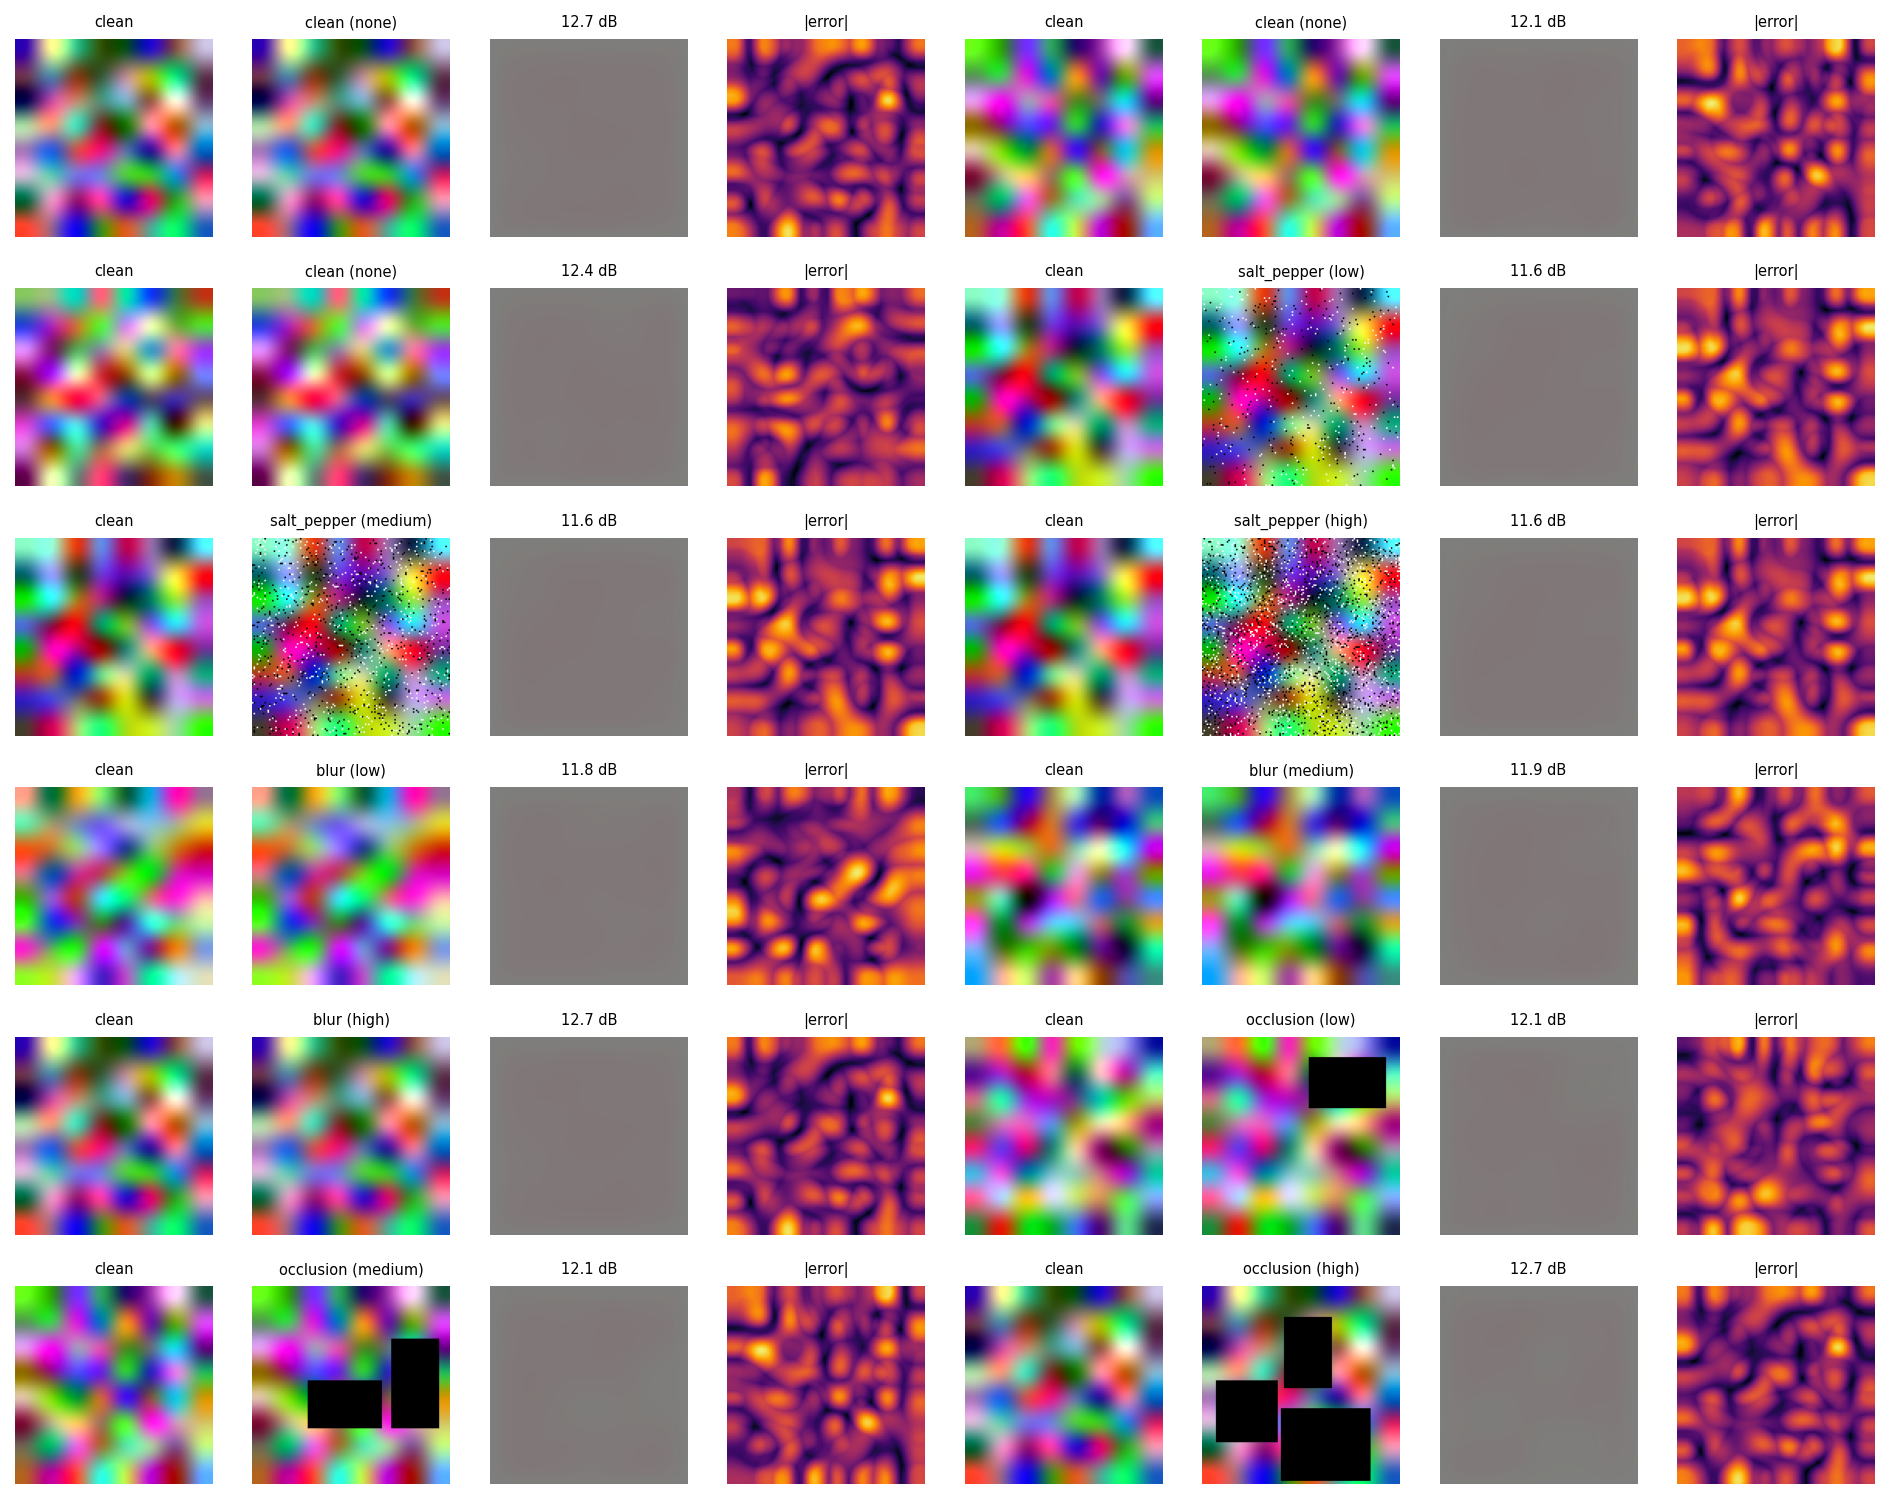
\includegraphics[width=0.92\textwidth]{t1_examples.png}
\caption{Task 1: twelve representative test examples (clean target, corrupted input, reconstruction with PSNR, absolute error map). Rows: clean inputs, then salt-and-pepper, blur and occlusion at low/medium/high severity.}
\label{fig:t1ex}
\end{figure*}

\begin{figure}[t]
\centering
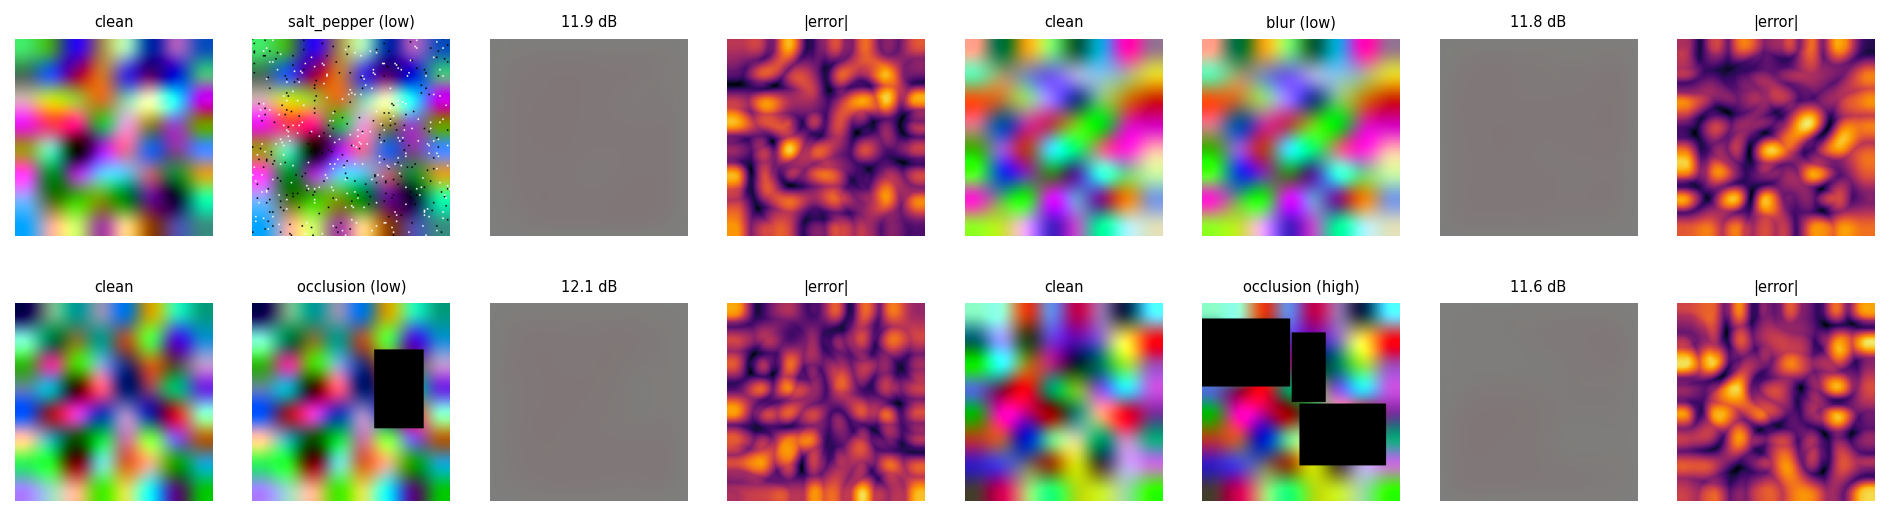
\includegraphics[width=\columnwidth]{t1_failures.png}
\caption{Task 1 failure cases (lowest PSNR gain per corruption type and lowest SSIM overall).}
\label{fig:t1fail}
\end{figure}

\textbf{Failure cases} (Fig.~\ref{fig:t1fail}). (1) \emph{Image borders:} a photograph with a thin white/black frame and low-severity salt-and-pepper noise drops from 19.5 to 17.2\,dB, because the decoder cannot reproduce a sharp one-pixel frame through the bottleneck and smears it into a coloured halo. (2) \emph{Saturated flat backgrounds:} for a cat on a uniform purple background with mild blur, the DAE introduces colour shifts in the flat region (37.2$\to$24.8\,dB) --- the network has learned to ``sharpen'', which creates artefacts where there is nothing to sharpen. (3) \emph{Occluders on black backgrounds:} when a black mask falls on an already black background, the corruption is invisible, yet the network in-paints a bright, wrong colour into the dark region (38.1$\to$12.3\,dB); it has learned the shortcut ``large black area $\Rightarrow$ fill it'', a direct consequence of the black-occluder definition. (4) \emph{High-frequency structure under strong blur:} the slats of a fence blurred with $(7,2.5)$ cannot be recovered (18.1\,dB); the information is destroyed by the blur and the bottleneck cannot hallucinate a periodic pattern.
\begin{figure*}[t]
\centering
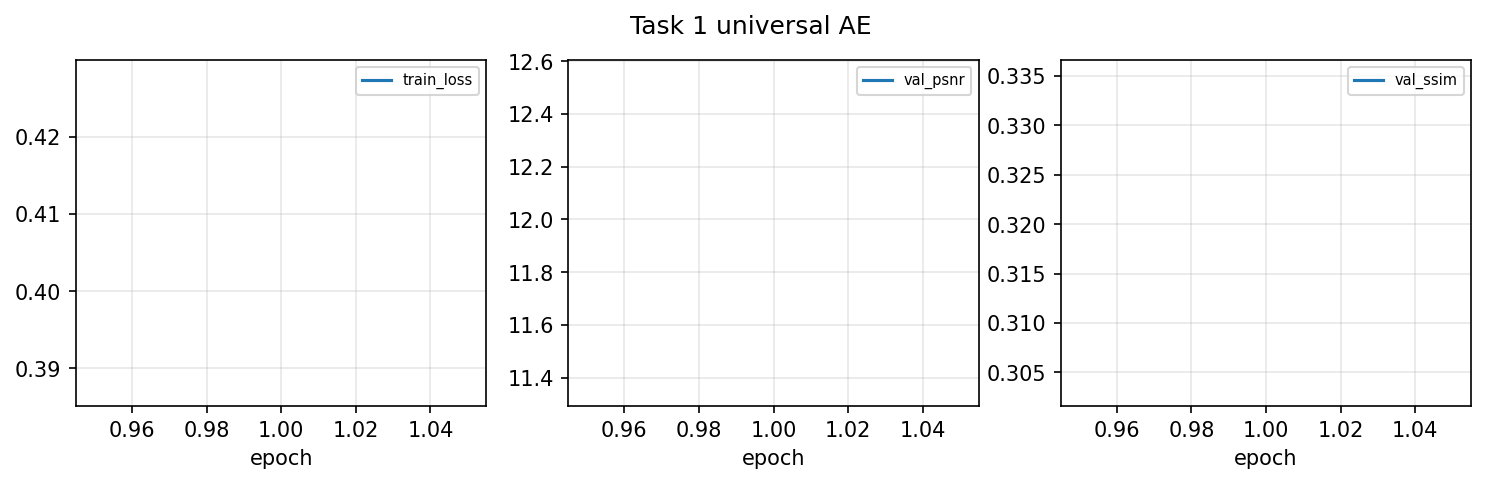
\includegraphics[width=0.49\textwidth]{t1_curves.png}\hfill
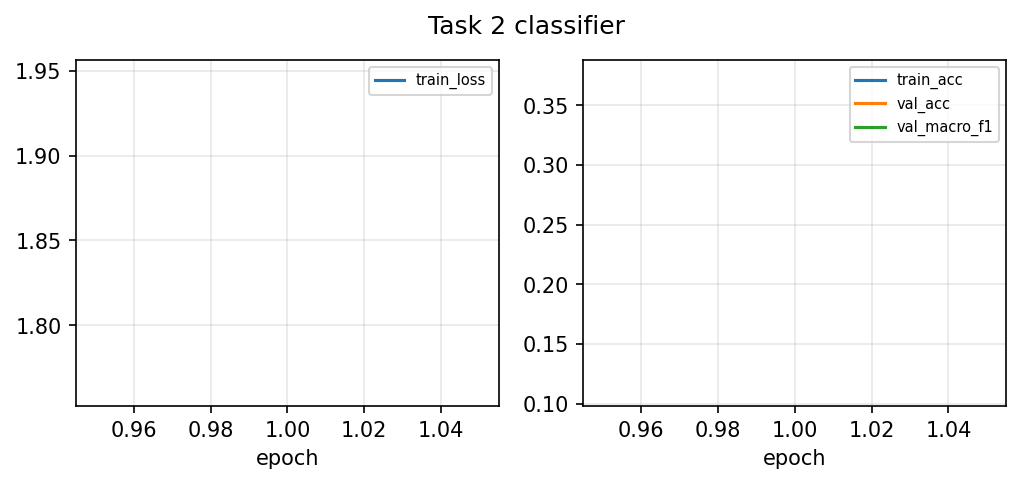
\includegraphics[width=0.49\textwidth]{t2_cls_curves.png}\\[1mm]
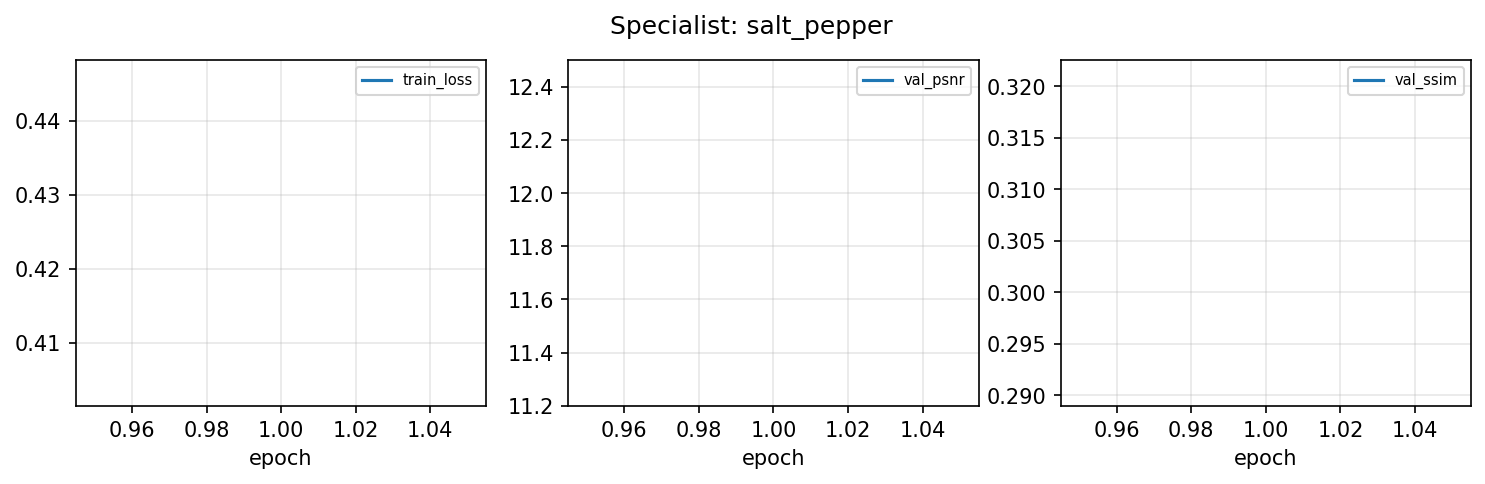
\includegraphics[width=0.49\textwidth]{t2_spec_salt_pepper_curves.png}\hfill
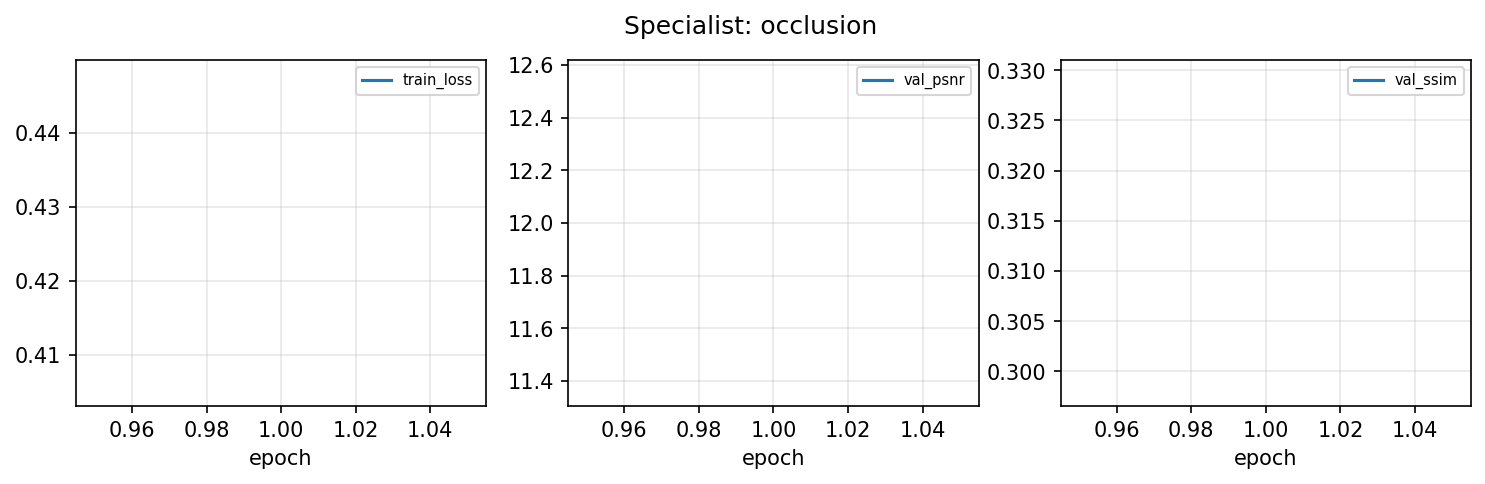
\includegraphics[width=0.49\textwidth]{t2_spec_occlusion_curves.png}\\[1mm]
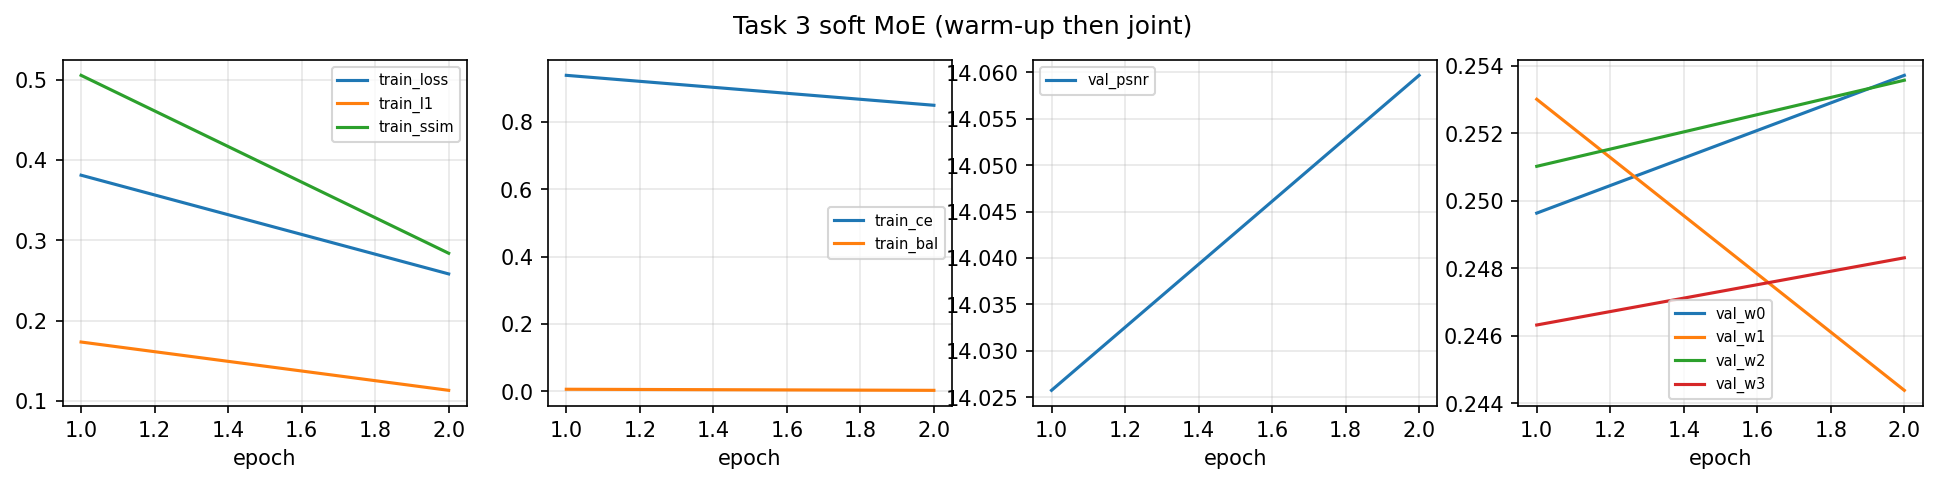
\includegraphics[width=0.98\textwidth]{t3_moe_curves.png}
\caption{Training and validation curves of the final runs: Task 1 universal DAE, Task 2 classifier, two of the Task 2 specialists (the blur specialist behaves alike), and Task 3 soft MoE (epochs 1--\MOEWARM: warm-up with frozen experts; afterwards joint fine-tuning; mean routing weights on the validation set in the last panel).}
\label{fig:curves}
\end{figure*}

\begin{figure*}[t]
\centering
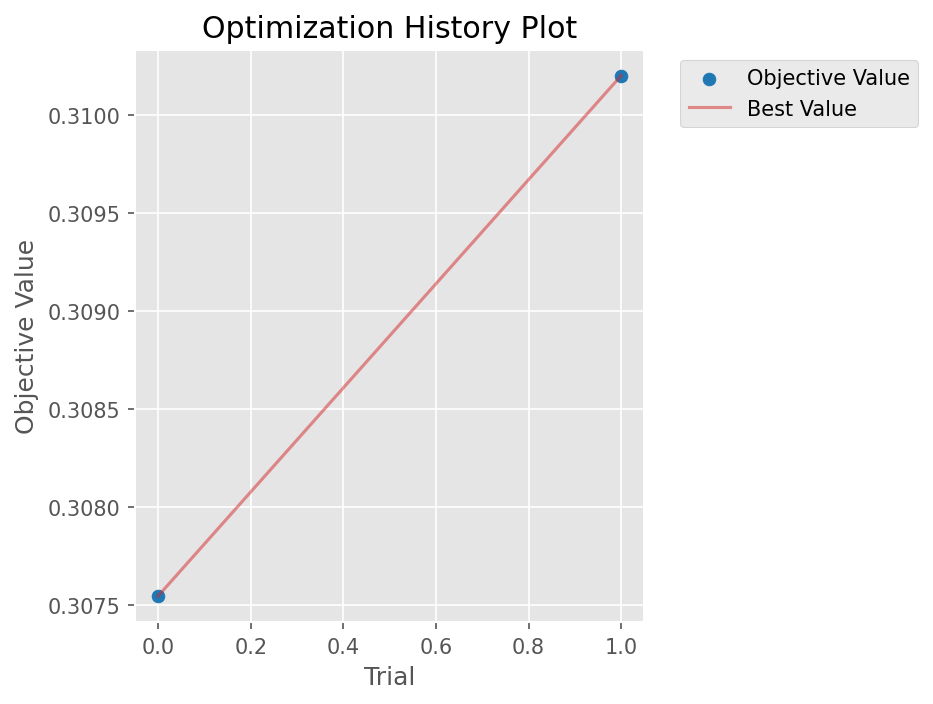
\includegraphics[width=0.24\textwidth]{optuna_t1_universal_ae_history.png}\hfill
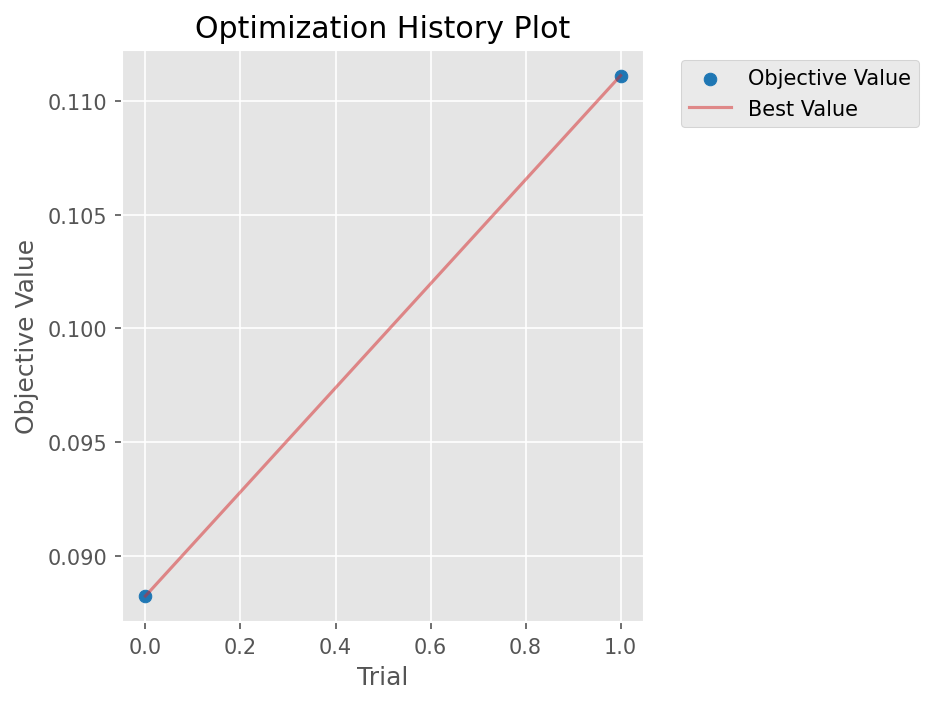
\includegraphics[width=0.24\textwidth]{optuna_t2_classifier_history.png}\hfill
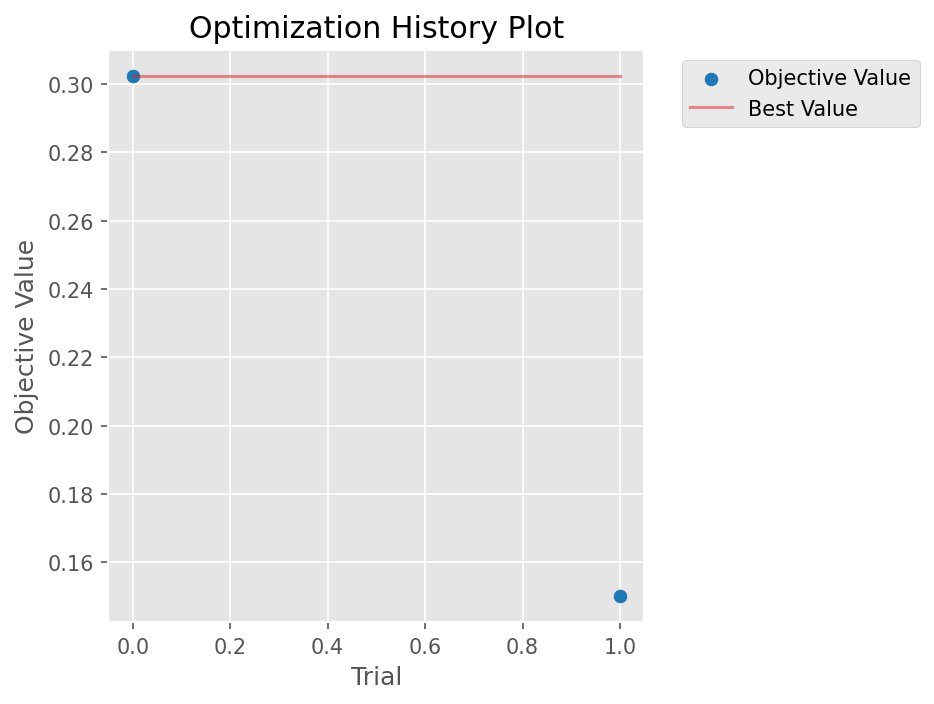
\includegraphics[width=0.24\textwidth]{optuna_t2_specialists_history.png}\hfill
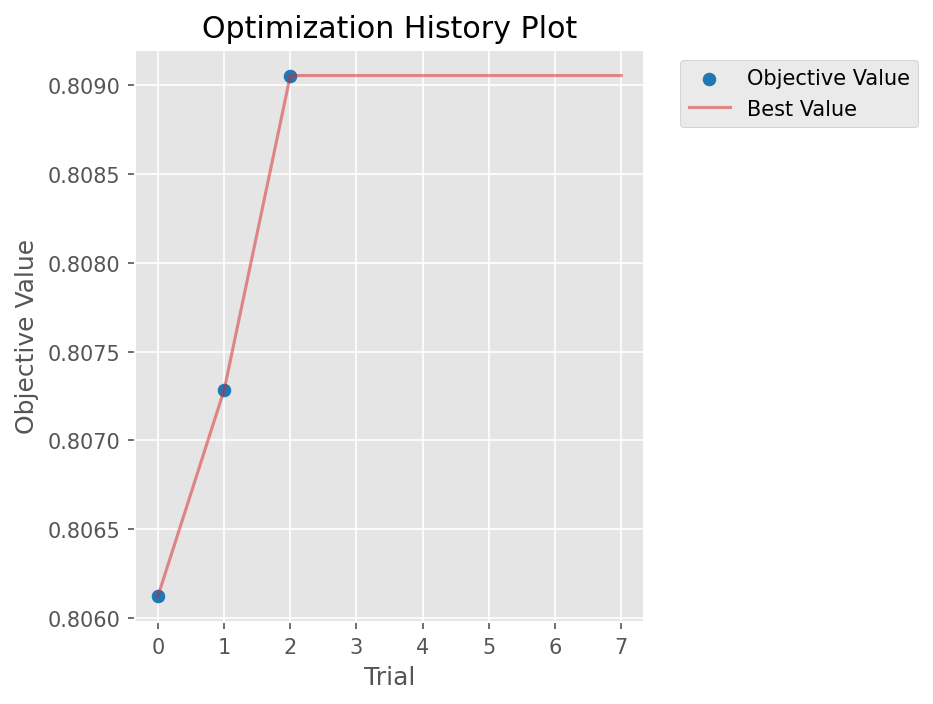
\includegraphics[width=0.24\textwidth]{optuna_t3_soft_moe_v2_history.png}\\[1mm]
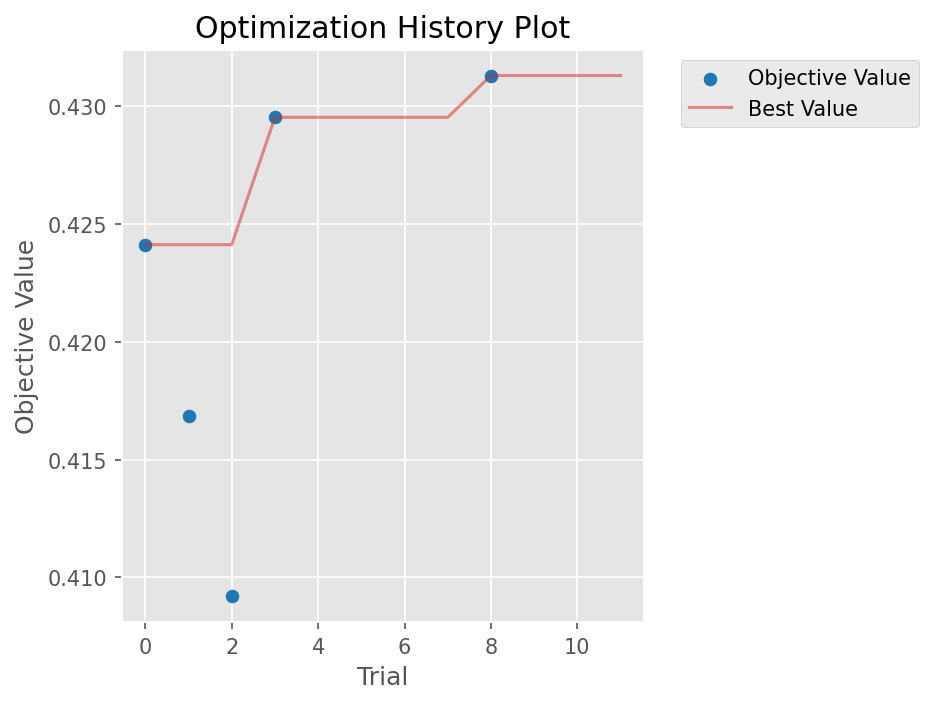
\includegraphics[width=0.24\textwidth]{optuna_t4_sketch_gan_history.png}\hfill
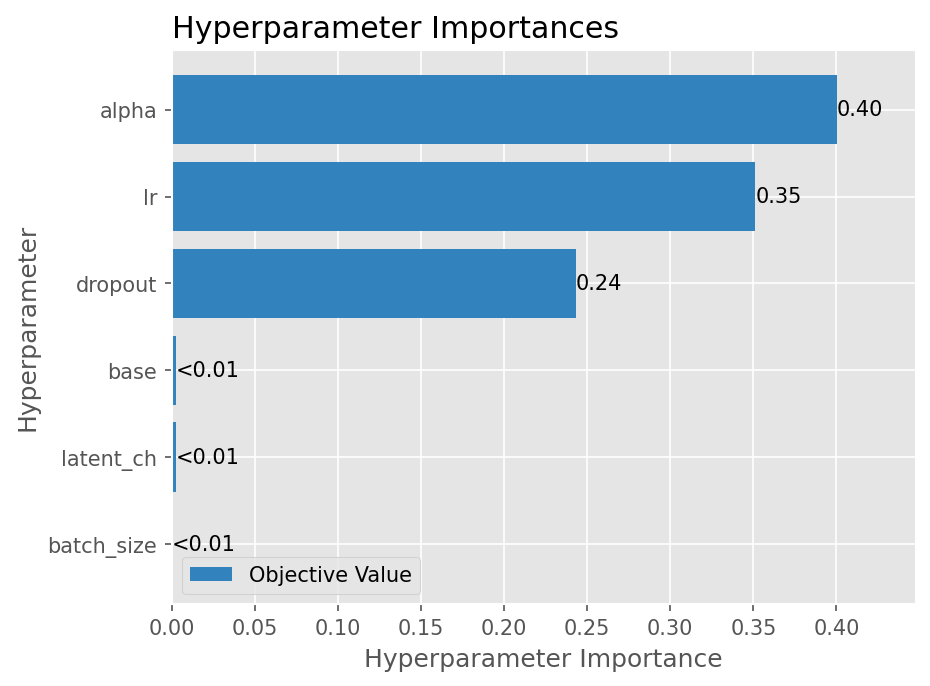
\includegraphics[width=0.24\textwidth]{optuna_t1_universal_ae_importance.png}\hfill
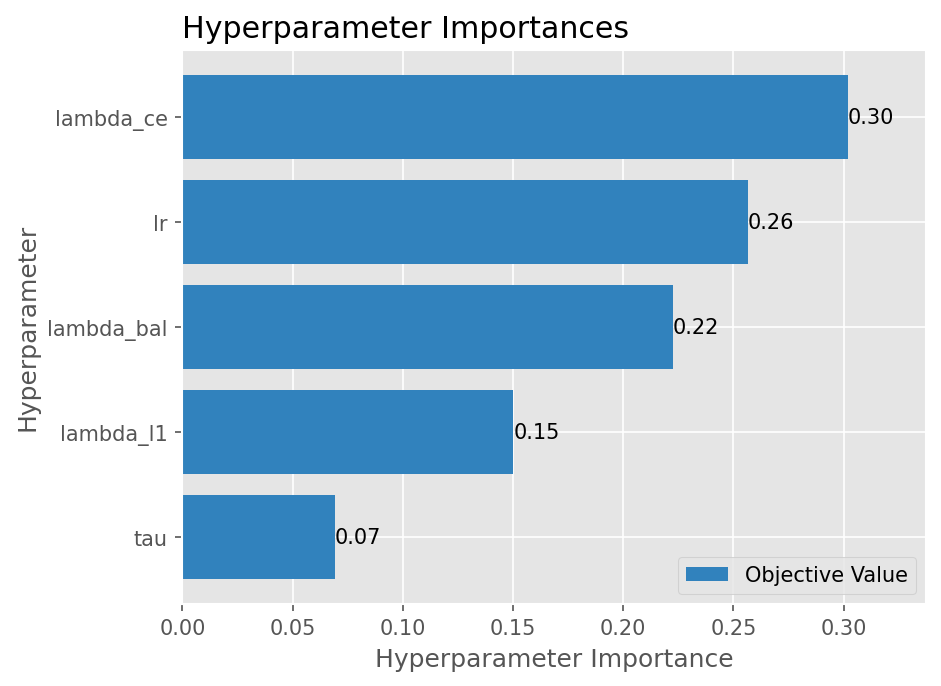
\includegraphics[width=0.24\textwidth]{optuna_t3_soft_moe_v2_importance.png}\hfill
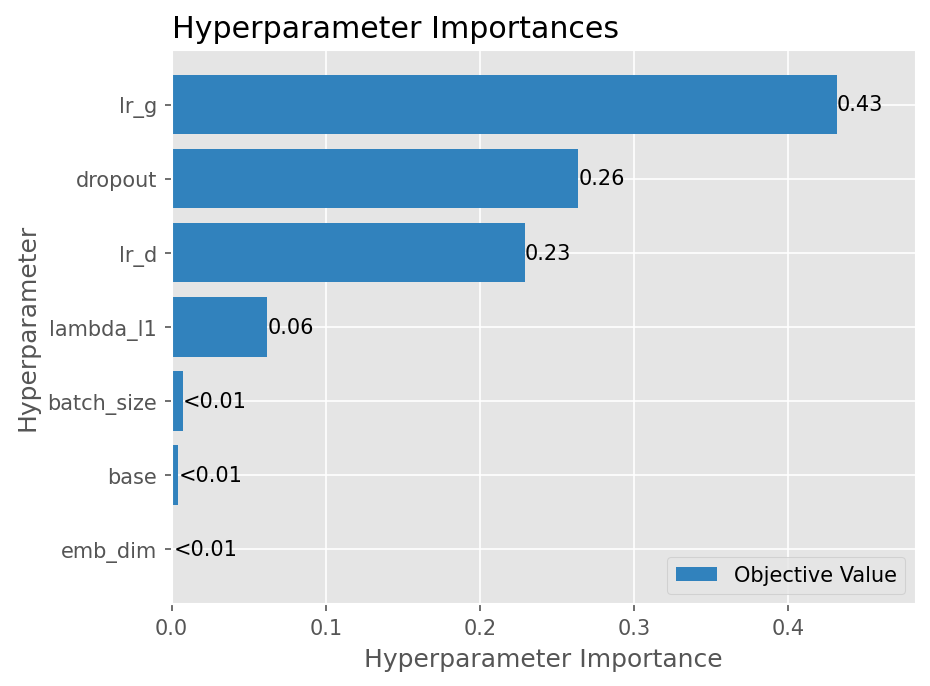
\includegraphics[width=0.24\textwidth]{optuna_t4_sketch_gan_importance.png}
\caption{Optuna studies. Top: optimisation histories of the Task 1 DAE, Task 2 classifier, Task 2 shared specialist search and Task 3 soft MoE. Bottom: Task 4 GAN history and fANOVA hyper-parameter importances for Tasks 1, 3 and 4 (importances use completed trials only).}
\label{fig:optuna}
\end{figure*}



%=====================================================================
\section{Task 2: Classification and Hard-Routed Specialists}
\subsection{Corruption classifier}
The classifier $C$ stacks 4--5 blocks of two $3\times3$ conv--BN--ReLU layers and $2\times2$ max-pooling. The first block works at full resolution because both blur and isolated impulses are high-frequency cues that early striding would erase. Global \emph{average} and global \emph{max} pooling are concatenated before dropout and a linear layer: max pooling preserves strong local evidence such as a single black rectangle or a few saturated pixels that average pooling would dilute. It is trained with cross-entropy on balanced batches (exactly $B/4$ samples per class), so the classifier cannot exploit a class prior. Optuna tuned the learning rate, batch size \{32,64,128\}, channel configuration \{small, medium, large\}, dropout $[0,0.5]$ and weight decay $[10^{-6},10^{-2}]$ (log), maximising validation macro-F1 (\CLSTRIALS{} trials; best: \CLSBESTPARAMS).

\subsection{Specialists}
The three specialists reuse the Task-1 architecture with independent parameters; each sees only its own corruption (the \texttt{classes} argument of the runtime dataset) and reconstructs the same clean target. To keep the search affordable, one shared Optuna study selected a common architecture: each trial trains all three specialists briefly and returns the mean of their validation objectives, so the chosen configuration is good for all three rather than for one. The search covered learning rate, bottleneck channels, base channels, batch size and $\alpha$ (\SPTRIALS{} trials; best: \SPBESTPARAMS). The three specialists were then trained independently for \SPEPOCHS{} epochs.

\subsection{Routing}
At inference $r=\arg\max_k p_k$; $r=\text{clean}$ returns $\tilde{x}$ unchanged (identity bypass), otherwise only the selected specialist is executed (Fig.~\ref{fig:routing}a). We evaluate \emph{oracle routing} (the manifest label selects the expert) and \emph{predicted routing} (the classifier selects it).

\subsection{Results}
\textbf{Classifier.} On the validation manifest the classifier reaches 99.73\,\% accuracy and 0.997 macro-F1; on the full test set (36{,}690 inputs) it reaches \textbf{99.87\,\%} accuracy, macro precision 0.998, macro recall 0.998 and macro-F1 \textbf{0.998} (Table~\ref{tab:cls}, Fig.~\ref{fig:cm}). Salt-and-pepper is recognised perfectly; all errors involve the clean class: 0.4\,\% of clean images are predicted as blur and 0.2\,\% as occlusion, and 0.2\,\% of occluded images are predicted as clean. Accuracy is 100\,\% at medium and high severity and 99.8\,\% at low severity, i.e.\ errors only occur where the corruption is weakest.

\begin{table}[t]
\centering
\caption{Classifier test metrics (36,690 test inputs)}
\label{tab:cls}
\begin{tabular}{lccc}
\toprule
Class & Precision & Recall & F1 \\
\midrule
Clean & 0.993 & 0.994 & 0.994 \\
Salt \& pepper & 1.000 & 1.000 & 1.000 \\
Gaussian blur & 0.999 & 1.000 & 0.999 \\
Occlusion & 0.999 & 0.998 & 0.999 \\
\midrule
Macro avg. & 0.998 & 0.998 & 0.998 \\
Accuracy & \multicolumn{3}{c}{0.9987} \\
\bottomrule
\end{tabular}
\end{table}

\begin{figure}[t]
\centering
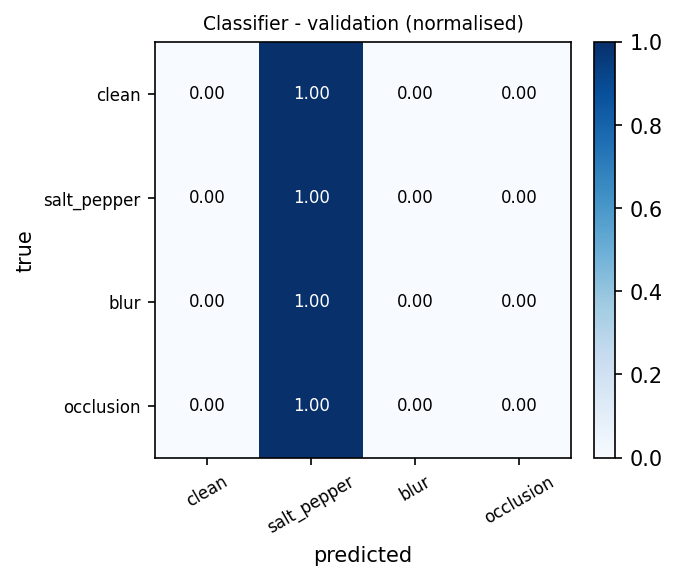
\includegraphics[width=0.49\columnwidth]{t2_confusion_val.png}\hfill
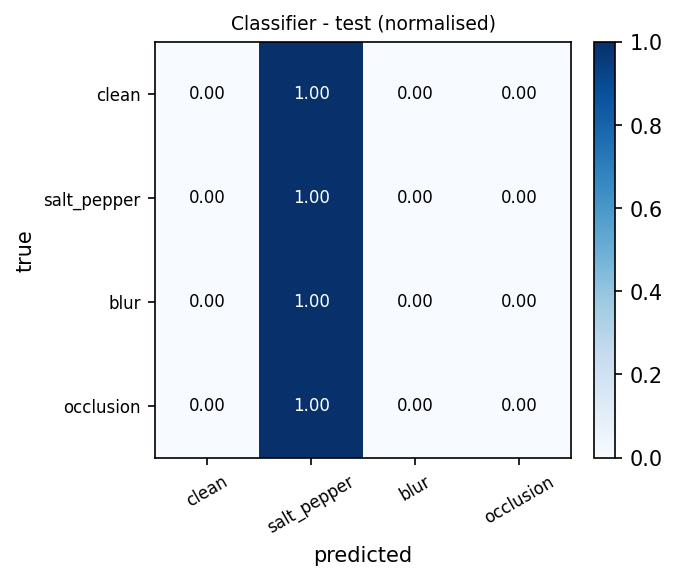
\includegraphics[width=0.49\columnwidth]{t2_confusion_test.png}
\caption{Normalised four-class confusion matrices of the corruption classifier on the validation (left) and test (right) manifests.}
\label{fig:cm}
\end{figure}

\textbf{Oracle vs.\ predicted routing.} Because the classifier is almost perfect, predicted routing is practically identical to oracle routing: 26.12 vs.\ 26.11\,dB and 0.808 vs.\ 0.808 SSIM over all corrupted inputs (Tables~\ref{tab:psnr_type}--\ref{tab:ssim_sev}). Only 46 of 36{,}690 inputs (0.13\,\%) were misrouted. Interestingly, predicted routing is marginally \emph{better} than oracle routing on low-severity occlusion (24.81 vs.\ 24.79\,dB): in the 25 occlusion$\to$clean errors the black mask lies on an already black region, so the occlusion is effectively invisible and the identity bypass returns a nearly perfect image, whereas the occlusion specialist would have in-painted a wrong colour.

\textbf{Misrouting failures} (Fig.~\ref{fig:misroute}). The harmful errors are the 21 clean images sent to an expert, which lose 13.6\,dB on average. They have a clear common cause: letter-boxed or framed photographs with \emph{black bars at the borders}. The classifier interprets the black bars as occluders and routes the image to the occlusion specialist, which then ``repairs'' the bars by painting them with background colour (11.6--12.8\,dB). The remaining clean$\to$blur errors are soft, low-contrast photographs that genuinely look slightly blurred. This shows that the occlusion definition (pure black rectangles) is ambiguous with naturally occurring black regions, and that a hard decision converts a small classification error into a large restoration error.

\begin{figure}[t]
\centering
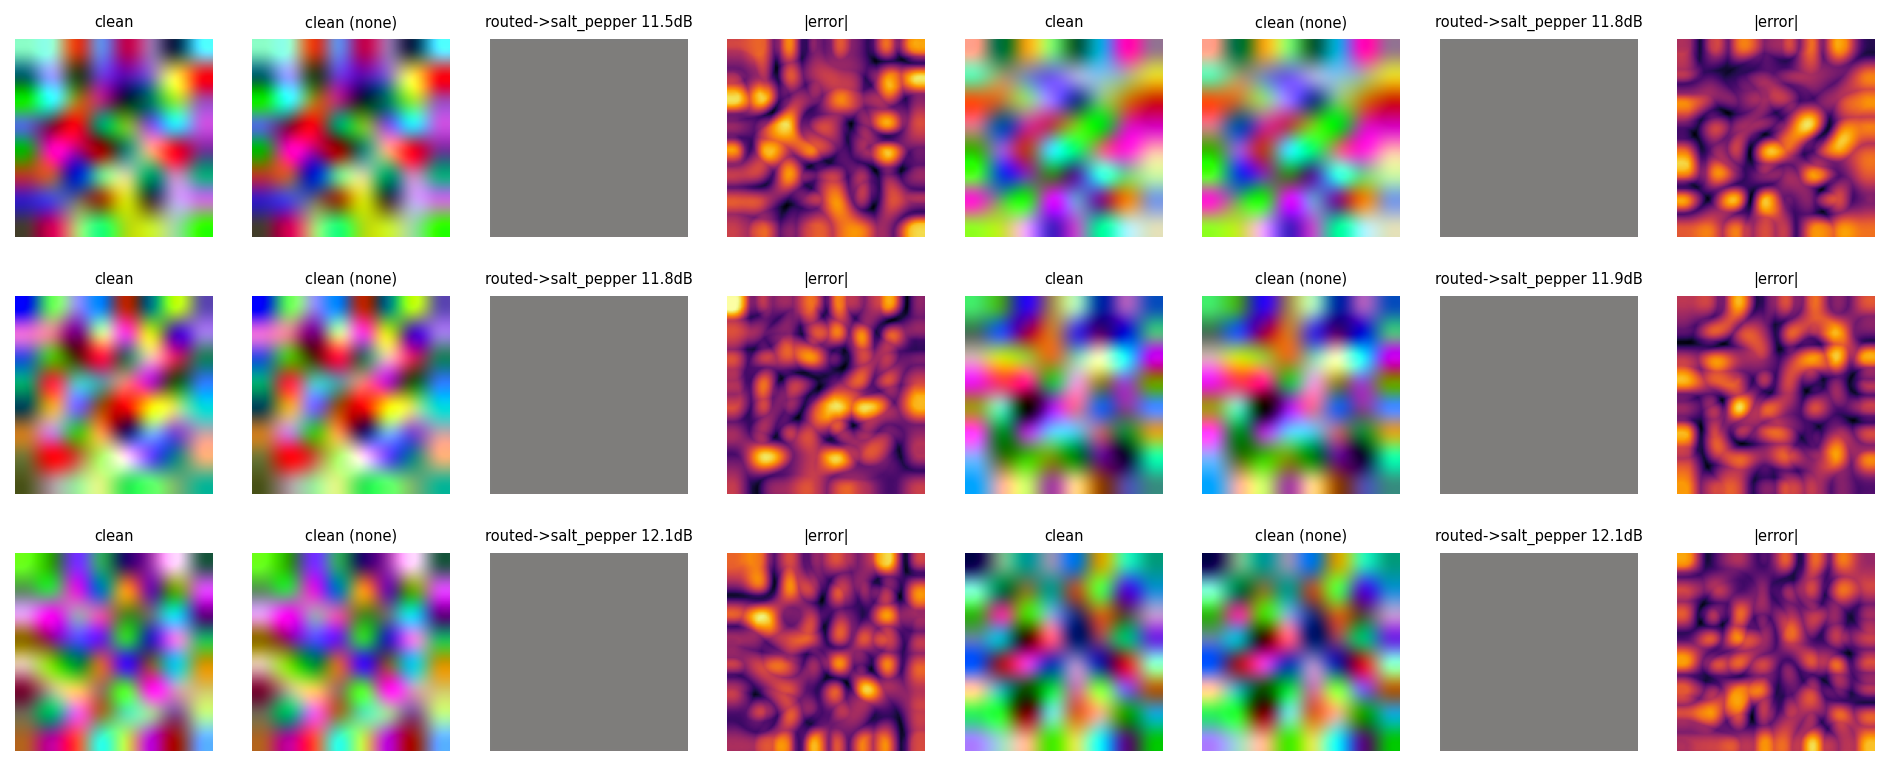
\includegraphics[width=\columnwidth]{t2_misrouted.png}
\caption{Predicted-routing failures with the largest PSNR loss: clean images with black borders are routed to the occlusion expert, which paints over the borders.}
\label{fig:misroute}
\end{figure}

\textbf{Specialists vs.\ universal model.} The comparison with Task 1 is instructive. With an identity bypass, clean images are returned unchanged (100\,dB / SSIM 1.0 under oracle routing; 99.6\,dB / 0.999 predicted) instead of being smoothed to 28.4\,dB, which is the single largest advantage of routing. On corrupted inputs, however, the specialists are \emph{not} clearly better than the universal DAE: they win on occlusion PSNR (22.80 vs.\ 22.37\,dB) and high blur (26.00 vs.\ 25.59\,dB) but lose slightly on salt-and-pepper (28.15 vs.\ 28.23\,dB) and on SSIM for every corruption (0.808 vs.\ 0.817 on average). Two factors explain this. First, both systems hit the same $\approx$28\,dB ceiling imposed by the bottleneck, so specialisation cannot help where the bottleneck, not the task diversity, is the limit. Second, the shared specialist search preferred a smaller encoder ($b=48$) and a larger L1 weight ($\alpha=0.77$ vs.\ 0.56), which trades SSIM for PSNR. In other words, the universal network had enough capacity to learn all three corruptions jointly at this resolution.


%=====================================================================
\section{Task 3: Jointly Trained Soft Mixture-of-Experts}
\subsection{Model}
The gate $G$ has the classifier architecture and is initialised with the trained Task-2 classifier; the experts are initialised with the three trained specialists (Fig.~\ref{fig:routing}b). For input $\tilde{x}$,
$w=\text{softmax}(G(\tilde{x})/\tau)$ and $\hat{x}=w_0\tilde{x}+w_1A_{salt}(\tilde{x})+w_2A_{blur}(\tilde{x})+w_3A_{occ}(\tilde{x})$. Because the combination is differentiable, the reconstruction error back-propagates into both the gate and the experts. The whole pipeline, including the softmax, the temperature and the weighted sum, is exported as one ONNX graph with two outputs (image and weights).

\begin{figure}[t]
\centering
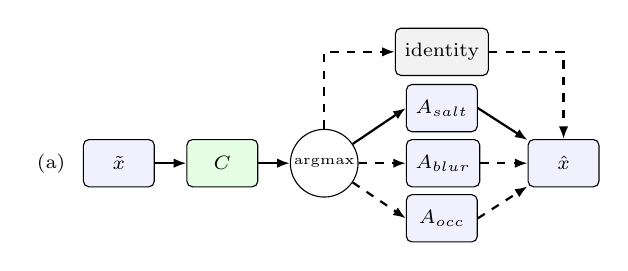
\begin{tikzpicture}[node distance=2mm]
\node[blk] (x) {$\tilde{x}$};
\node[blk, right=4mm of x, fill=green!10] (c) {$C$};
\node[op, right=4mm of c] (sw) {\tiny argmax};
\node[blk, right=6mm of sw, yshift=7mm] (a1) {$A_{salt}$};
\node[blk, right=6mm of sw] (a2) {$A_{blur}$};
\node[blk, right=6mm of sw, yshift=-7mm] (a3) {$A_{occ}$};
\node[blk, above=1mm of a1, fill=gray!10] (id) {identity};
\node[blk, right=6mm of a2] (o) {$\hat{x}$};
\draw[arr] (x)--(c); \draw[arr] (c)--(sw);
\draw[arr, dashed] (sw.north) |- (id.west); \draw[arr] (sw)--(a1.west); \draw[arr, dashed] (sw)--(a2.west); \draw[arr, dashed] (sw)--(a3.west);
\draw[arr] (a1.east)--(o); \draw[arr, dashed] (id.east) -| (o.north); \draw[arr, dashed] (a2)--(o); \draw[arr, dashed] (a3.east)--(o);
\node[font=\scriptsize, left=1mm of x] {(a)};
\end{tikzpicture}\\[2mm]
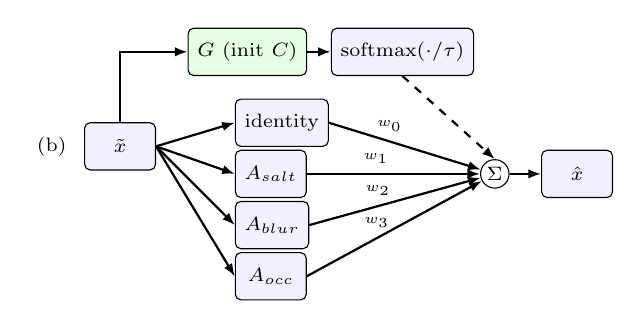
\begin{tikzpicture}[node distance=2mm]
\node[blk] (x) {$\tilde{x}$};
\node[blk, right=4mm of x, fill=green!10, yshift=12mm] (g) {$G$ (init $C$)};
\node[blk, right=3mm of g] (sm) {softmax$(\cdot/\tau)$};
\node[blk, right=10mm of x, yshift=3mm] (id) {identity};
\node[blk, right=10mm of x, yshift=-3.5mm] (a1) {$A_{salt}$};
\node[blk, right=10mm of x, yshift=-10mm] (a2) {$A_{blur}$};
\node[blk, right=10mm of x, yshift=-16.5mm] (a3) {$A_{occ}$};
\node[op, right=22mm of a1] (sum) {$\Sigma$};
\node[blk, right=4mm of sum] (o) {$\hat{x}$};
\draw[arr] (x) |- (g); \draw[arr] (g)--(sm);
\foreach \n/\w in {id/w_0,a1/w_1,a2/w_2,a3/w_3} {\draw[arr] (x.east) -- (\n.west); \draw[arr] (\n.east) -- node[font=\tiny, above, pos=0.4] {$\w$} (sum);}
\draw[arr, dashed] (sm.south) -- (sum.north);
\draw[arr] (sum)--(o);
\node[font=\scriptsize, left=1mm of x] {(b)};
\end{tikzpicture}
\caption{(a) Hard routing: only the expert chosen by the classifier runs (dashed = not executed for this input). (b) Soft MoE: all branches run and are blended with gate weights $w$; gate and experts are trained jointly.}
\label{fig:routing}
\end{figure}

\subsection{Loss and two-stage training}
$\mathcal{L}_{MoE}=\lambda_1\mathcal{L}_{L1}+\lambda_s(1-\text{SSIM})+\lambda_c\mathcal{L}_{CE}(G(\tilde{x}),y)+\lambda_b\mathcal{L}_{balance}$, with $\mathcal{L}_{balance}=\sum_{k=0}^{3}(\bar{w}_k-\tfrac14)^2$ computed on balanced batches, where the ideal average weight of each branch is exactly $\tfrac14$. The cross-entropy term keeps the gate semantically tied to the corruption label, while the balance term (cf.\ the auxiliary load-balancing losses of~\cite{shazeer2017,fedus2021switch}) penalises collapse onto one branch. Note that, unlike in sparse MoE language models, here the balance term only acts on the \emph{batch mean}; per-sample weights remain free to be sharp, which is what we want. Training starts with a \MOEWARM-epoch warm-up in which the experts are frozen (parameters \texttt{requires\_grad=False}, BN in eval mode) and only the gate is trained ($\text{lr}=10^{-4}$); afterwards all parameters are fine-tuned jointly with a smaller, Optuna-selected learning rate for \MOEEPOCHS{} epochs.

\subsection{Optuna study}
The joint learning rate $[10^{-5},3\cdot10^{-4}]$ (log), $\tau\in[0.5,2]$, $\lambda_c\in[0.01,0.5]$ (log), $\lambda_b\in[10^{-3},0.1]$ (log) and the reconstruction weighting $\lambda_1\in[0.5,0.95]$ with $\lambda_s=1-\lambda_1$ were searched (\MOETRIALS{} trials). Besides median pruning we added a domain-specific pruning rule: a trial is stopped as soon as the mean validation weight of any branch falls below 0.02, i.e.\ when routing collapses (\MOECOLLAPSED{} trials were pruned this way). Selected: \MOEBESTPARAMS.

\subsection{Results}
\textbf{A model-selection pitfall and its fix.} Our first MoE run (v1) selected checkpoints with $S$ computed from the \emph{mean} PSNR of the validation set. Because the identity branch returns clean images almost unchanged, their PSNR is $\approx$100\,dB, and these few values dominated the mean: the validation mean PSNR fell from 39.3 to $\approx$36.8\,dB as soon as joint fine-tuning started, although SSIM \emph{rose} from 0.865 to 0.871. The criterion therefore kept the end of the warm-up (experts still frozen) as the ``best'' model, the v1 MoE was in effect hard routing with a re-trained gate (corrupted inputs 26.17\,dB / 0.811 SSIM, routing entropy 0.07, 97\,\% of inputs with $\max_k w_k>0.9$), and the joint fine-tuning had been discarded. We found this by inspecting the per-epoch history rather than only the final numbers. The fix caps PSNR at 40\,dB \emph{per image} before averaging; the whole MoE stage (Optuna search and final training) was then re-run (v2) from the same Task-2 checkpoints. All MoE results below are from v2; the v1 study is kept in the repository as evidence.

\textbf{Reconstruction.} With the corrected criterion the best checkpoint is the last joint epoch (Fig.~\ref{fig:curves}, bottom): validation SSIM rises from 0.871 after warm-up to 0.884, so joint fine-tuning now clearly helps. On the test set the soft MoE is the best system on corrupted inputs, with \MOEPSNRCORR\,dB / \MOESSIMCORR{} SSIM versus \TONEPSNRCORR\,dB / \TONESSIMCORR{} (universal DAE) and \PREDPSNRCORR\,dB / \PREDSSIMCORR{} (predicted hard routing). It is best in SSIM for every corruption and severity (Table~\ref{tab:ssim_sev}) and best in PSNR for all blur and salt-and-pepper levels. The largest gains appear exactly where the bottleneck hurt the other systems: low blur (29.7\,dB / 0.901 vs.\ 28.1 / 0.857 for hard routing) and low occlusion (SSIM 0.881 vs.\ 0.805). Clean images keep near-identity quality (58.5\,dB, SSIM 0.999). The only regression is occlusion PSNR at medium/high severity (20.56 vs.\ 20.77\,dB at high severity), discussed below.

\begin{figure}[t]
\centering
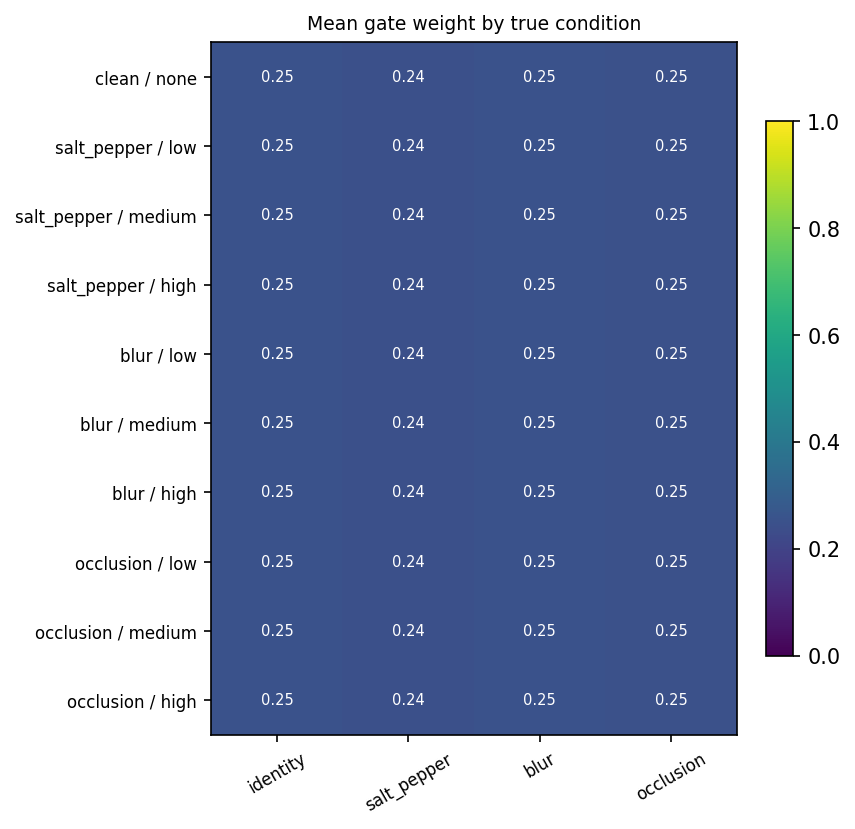
\includegraphics[width=0.85\columnwidth]{t3_routing_heatmap.png}
\caption{Routing heatmap: mean gate weight of each branch for every true corruption and severity on the test set.}
\label{fig:heat}
\end{figure}

\begin{figure*}[t]
\centering
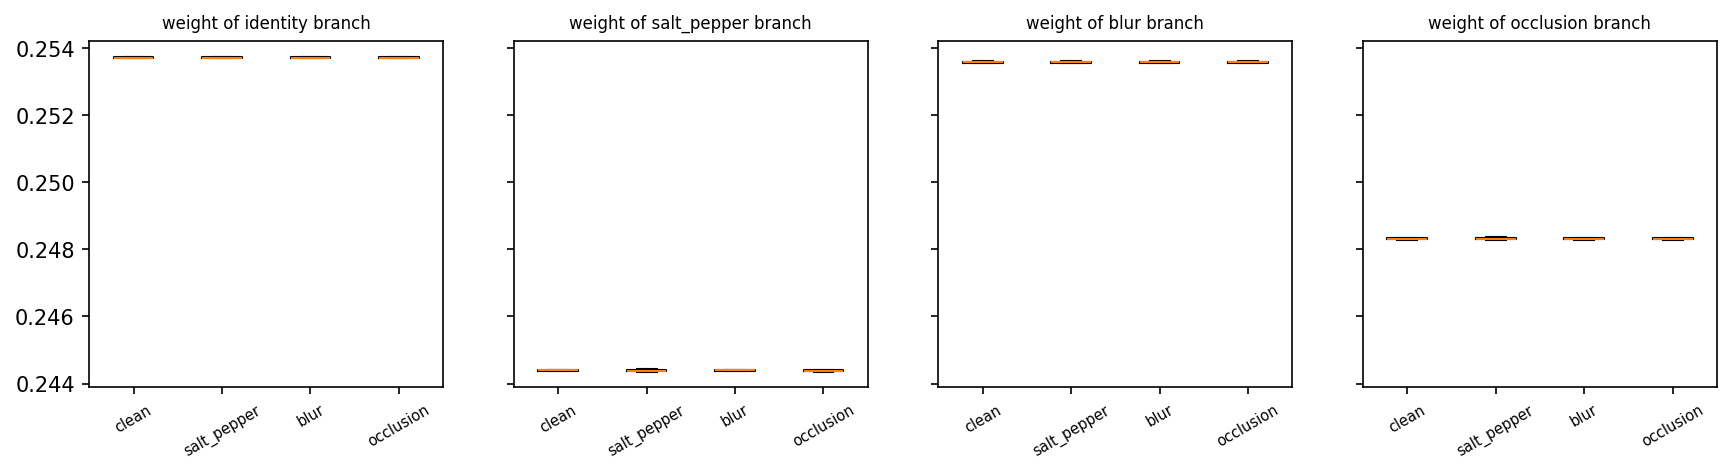
\includegraphics[width=0.98\textwidth]{t3_weight_distribution.png}
\caption{Distribution of the four routing weights per true input condition (test set, box = inter-quartile range).}
\label{fig:wdist}
\end{figure*}

\textbf{Routing behaviour} (Figs.~\ref{fig:heat}, \ref{fig:wdist}). The gate remains semantically aligned with the corruption: the matching branch receives the largest weight for clean (0.96), salt-and-pepper (0.89--0.96), blur (0.65--0.87) and occlusion (0.56--0.73) inputs, and the argmax of $w$ agrees with the true label for 96.7\,\% of test inputs. No expert is inactive (overall mean weights 0.27/0.28/0.25/0.20), and no expert dominates unrelated inputs: the salt-and-pepper, blur and occlusion experts receive on average only 0.0002, 0.019 and 0.008 of the weight on inputs that are not of their type. The only branch used on unrelated inputs is the \emph{identity} branch (0.19 on average for corrupted inputs) --- and this is the key learned behaviour. The identity weight decreases monotonically with severity (blur: 0.33/0.16/0.13; occlusion: 0.44/0.32/0.27; salt-and-pepper: 0.06/0.02/0.01): for mild corruptions the gate blends a sizeable fraction of the (almost clean) input with the expert's smoothed reconstruction, which restores the high-frequency detail that the bottleneck removes. This is effectively a learned, input-adaptive skip connection that hard routing cannot express. It already appears when only the gate is trained with the higher temperature of v2 (mean validation identity weight 0.32 after warm-up, where 0.25 would correspond to clean inputs only) and is strengthened by joint fine-tuning (0.38, Fig.~\ref{fig:curves}), during which the experts adapt to being blended. The routing entropy increased from 0.07 (v1) to 0.45, and only 35\,\% of inputs now have one branch with $w>0.9$.

\begin{figure}[t]
\centering
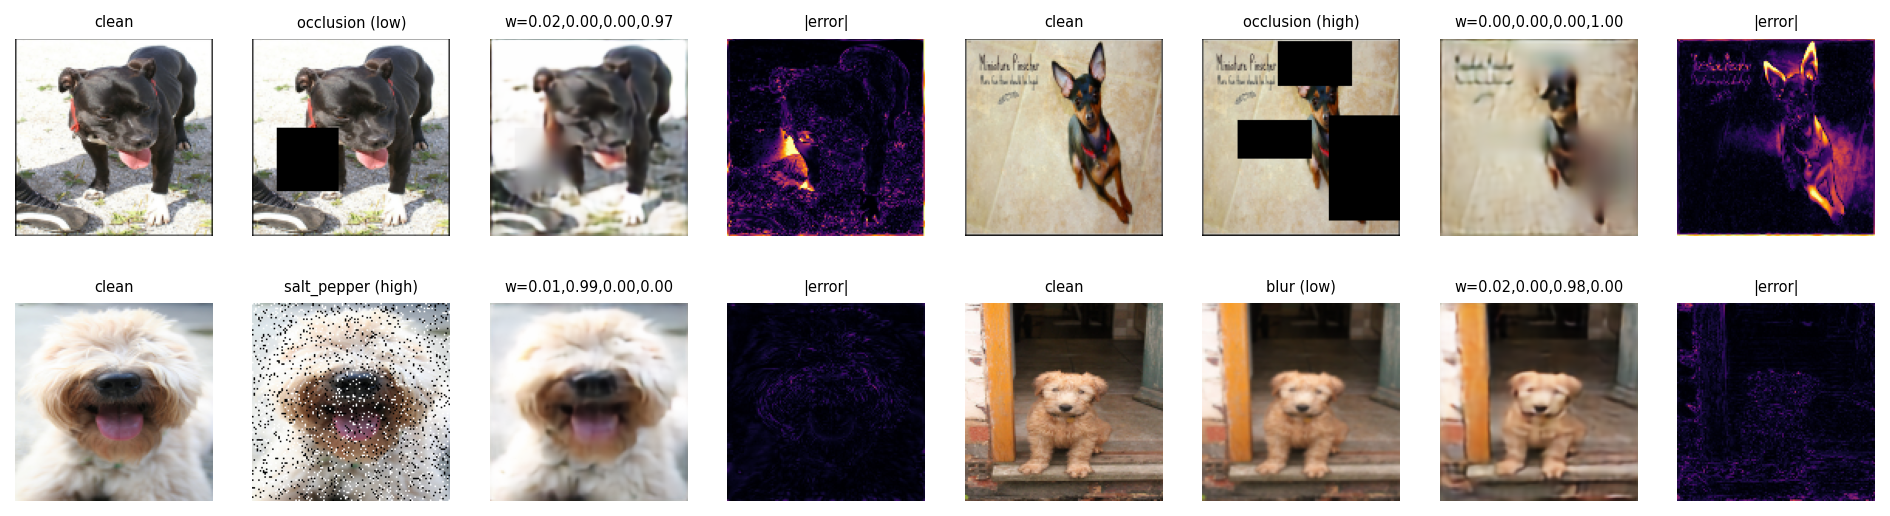
\includegraphics[width=\columnwidth]{t3_dominant_examples.png}\\[1mm]
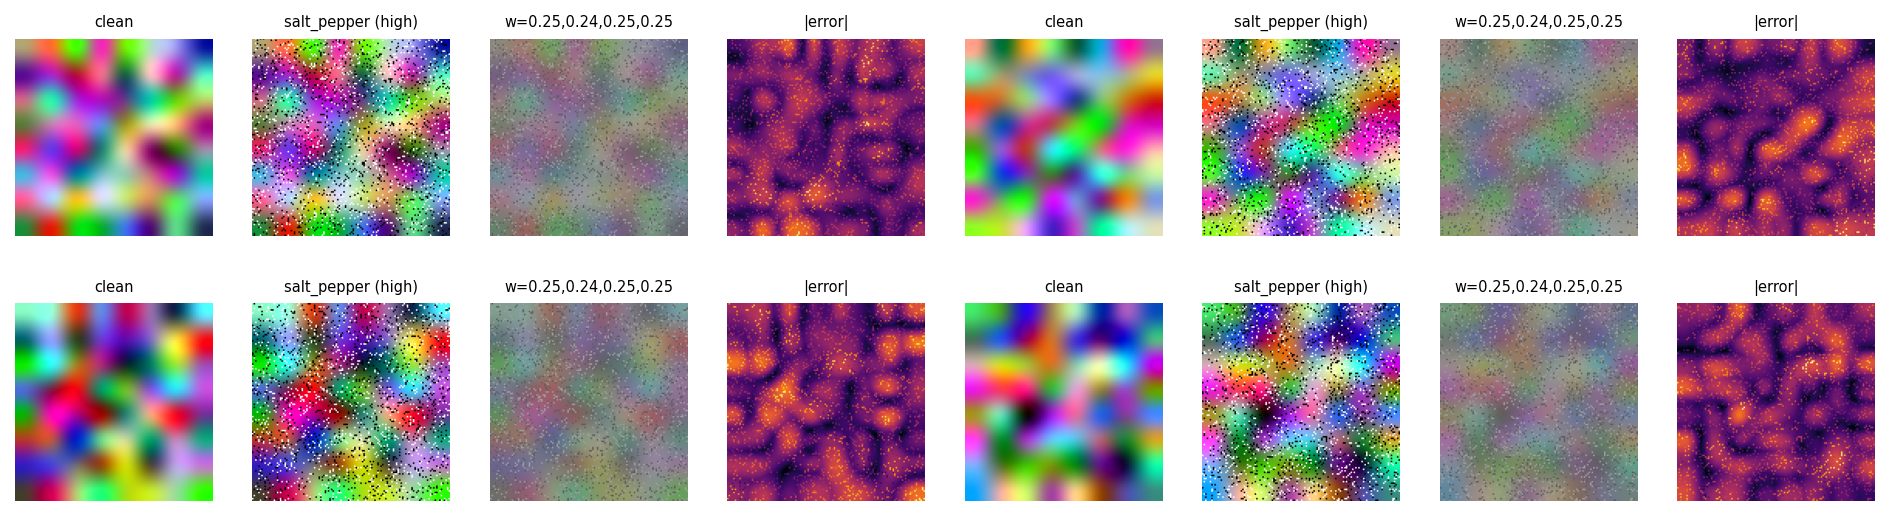
\includegraphics[width=\columnwidth]{t3_distributed_examples.png}
\caption{Top: inputs where one expert dominates ($w>0.9$). Bottom: inputs with the most distributed weights ($w=[w_0,w_1,w_2,w_3]$ in each title).}
\label{fig:moeex}
\end{figure}

\textbf{Dominant vs.\ distributed examples} (Fig.~\ref{fig:moeex}). Strong salt-and-pepper noise is handled almost exclusively by the salt-and-pepper expert ($w_1\approx0.95$; the blur expert receives a small, consistent 0.03--0.05). The most distributed weights occur for \emph{low}-severity salt-and-pepper on highly textured images (grass, flowers), where the gate splits $\approx$0.45/0.50 between identity and the salt-and-pepper expert: the texture makes the sparse impulses hard to distinguish from image detail. This is also a failure mode of soft routing --- blending 45\,\% of the input re-introduces faint impulses, visible as dots in the error maps. The same mechanism explains the occlusion regression: blending 27--44\,\% identity darkens the in-painted region again, which lowers PSNR inside large masks although SSIM, dominated by the unoccluded area, improves.

\textbf{Mixed corruptions.} To test the motivation of soft routing, we applied blur $(5,1.5)$ followed by salt-and-pepper $p=0.08$ --- a combination never seen in training --- to 300 test images. The classifier labels all of them as salt-and-pepper and the gate also concentrates on that expert ($w_1=0.95$, $w_2=0.04$). The MoE (25.8\,dB / 0.776) is only marginally better than hard routing (25.7\,dB / 0.771), while the universal DAE is clearly best (27.0\,dB / 0.821). Soft routing alone therefore does not solve compound degradations: the gate was never shown such inputs and the experts are applied in parallel, not in sequence, so no weighted sum of single-corruption experts can undo both corruptions. The universal model, which shares one representation across corruptions, generalises better here.

\textbf{Optuna.} Three of the eight v2 trials completed and five were pruned by the median rule; none had to be stopped by the routing-collapse rule, because the classifier initialisation and the cross-entropy term keep the gate aligned from the start. The search separates cleanly by temperature: all three completed trials used $\tau\ge1.6$ and all five pruned trials $\tau\le1.29$. The selected configuration (\MOEBESTPARAMS) uses a learning rate near the top of the range, a high temperature (softer weights) and small classification and balance weights, which is consistent with the observed benefit of softer, blended routing.


%=====================================================================
\section{Task 4: Style-Conditioned Face-to-Sketch GAN}
\subsection{Data}
We use the official FS2K split~\cite{fan2022fs2k} (\FSTRAINFULL{} training, \FSTEST{} test pairs). Fifteen percent of the training pairs, stratified by style with seed 42, form the validation set (\FSTRAIN/\FSVAL; validation styles \FSVALSTYLES). Photographs and sketches are resized to $128\times128$; the sketch of \texttt{photo1/image0110} is \texttt{sketch1/sketch0110}, and we verified the pairing visually. Augmentation uses the pix2pix jitter (resize to 142, random $128$ crop) and horizontal flips, applied with \emph{identical} parameters to both images of a pair to preserve pixel correspondence.

\subsection{Architecture}
The generator is a 7-level U-Net~\cite{ronneberger2015,isola2017} ($128\to1$, channels $b$ to $8b$, dropout in the three innermost decoder blocks). The style $s\in\{0,1,2\}$ is mapped by a learned \texttt{nn.Embedding} to $e_s\in\mathbb{R}^{d}$, which is broadcast spatially and concatenated (i) to the input photograph and (ii) to the $2\times2$ bottleneck features, so it controls both low-level stroke texture and global appearance. The discriminator is a PatchGAN~\cite{isola2017} that receives the photograph, a real or generated sketch and its own style embedding map, and outputs a $14\times14$ grid of real/fake logits, each judging a $70\times70$-pixel receptive field. Skip connections are appropriate here (unlike Tasks 1--3) because the sketch must align pixel-wise with the photograph.

\subsection{Objective and training}
With BCE-with-logits, $\mathcal{L}_D=\tfrac12[\text{BCE}(D(x,y,s),1)+\text{BCE}(D(x,G(x,s),s),0)]$ and $\mathcal{L}_G=\text{BCE}(D(x,G(x,s),s),1)+\lambda_{L1}\lVert y-G(x,s)\rVert_1$. Adam ($\beta_1=0.5$) with a constant learning rate for the first half of training and linear decay to zero afterwards follows pix2pix. Discriminator real loss, discriminator fake loss, generator adversarial loss, generator L1 loss and validation PSNR/SSIM/L1 are logged separately every epoch, and a fixed grid of six validation photographs (two per style) rendered in all three styles is logged every 10 epochs.

\subsection{Optuna study}
Generator and discriminator learning rates, batch size \{4,8,16\}, base channels \{32,48,64\}, dropout $[0,0.5]$, embedding dimension \{4,8,16\} and $\lambda_{L1}\in[10,200]$ (log) were searched with \FSTRIALS{} trials of \FSTRIALEP{} epochs; the best configuration (\FSBESTPARAMS) was retrained for \FSEPOCHS{} epochs. The validation objective is the same $S$ as in Task~1.

\subsection{Results}
\textbf{Training dynamics} (Fig.~\ref{fig:gancurves}). After a short transient in the first epochs, the discriminator real and fake losses settle at $\approx$0.53 and $\approx$0.51 and the generator adversarial loss decreases slowly from 1.2 to 1.05: neither network overpowers the other and there is no sign of mode collapse. The Optuna history (Fig.~\ref{fig:optuna}) shows that the reconstruction weight was the decisive hyper-parameter: all seven pruned trials used $\lambda_{L1}\le72$, all five completed ones $\lambda_{L1}\ge78$, independent of the learning rates. Part of this preference is built into the selection criterion, which is pixel-based (SSIM/PSNR) and therefore rewards a strong L1 term; a perceptual criterion might favour a smaller $\lambda_{L1}$. Among the completed trials the fANOVA importance attributes most of the variance to lr$_G$ (0.43), dropout (0.26) and lr$_D$ (0.23) and almost none to $\lambda_{L1}$ (0.06); this does not contradict the previous observation, because importance is computed on completed trials only, which all had a large $\lambda_{L1}$. The selected configuration uses $\lambda_{L1}=111$ (close to the pix2pix default of 100), lr$_G=4.0\cdot10^{-4}$ with a $9\times$ smaller lr$_D=4.5\cdot10^{-5}$, a large decoder dropout (0.47) and the largest embedding ($d=16$). The training L1 keeps decreasing until epoch 200 while the validation L1 flattens after $\approx$120 epochs, indicating mild over-fitting; the best validation objective was reached at epoch 168, whose weights are used.

\begin{figure}[t]
\centering
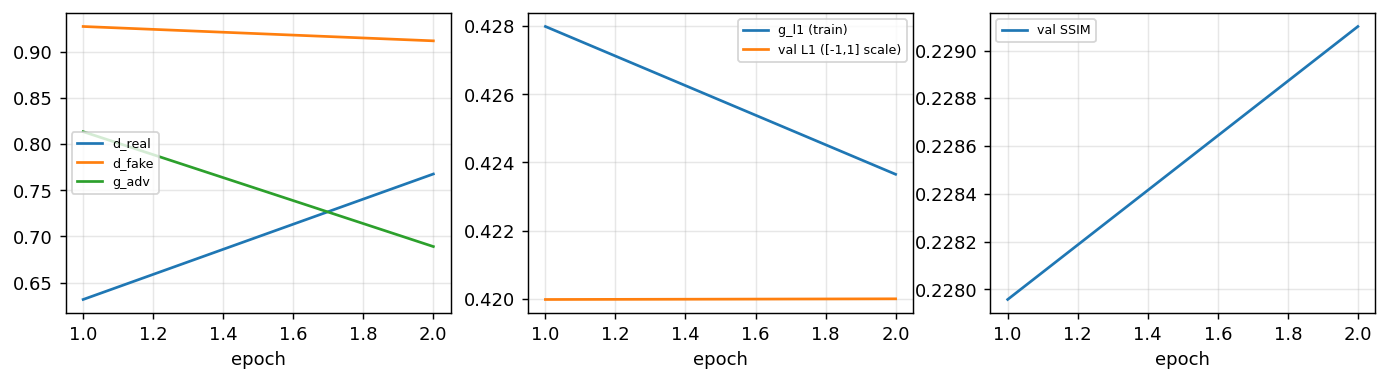
\includegraphics[width=\columnwidth]{t4_curves.png}
\caption{Task 4 training: discriminator real/fake loss and generator adversarial loss (left), generator L1 on training and validation data (middle), validation SSIM (right).}
\label{fig:gancurves}
\end{figure}

\textbf{Test results.} On the 1{,}046 official FS2K test pairs the generator reaches SSIM 0.480, PSNR 15.4\,dB and L1 0.107 (images in $[0,1]$). Results differ strongly by style: style~3 (light pencil) 0.625 / 18.5\,dB, style~1 (clean line drawing) 0.522 / 17.1\,dB and style~2 (dense charcoal shading) 0.393 / 12.3\,dB. Pixel metrics are a harsh measure for sketches: a stroke drawn two pixels away from the artist's stroke is penalised twice, although perceptually it is equally valid, so these numbers should be read as relative rather than absolute quality indicators.

\begin{figure}[t]
\centering
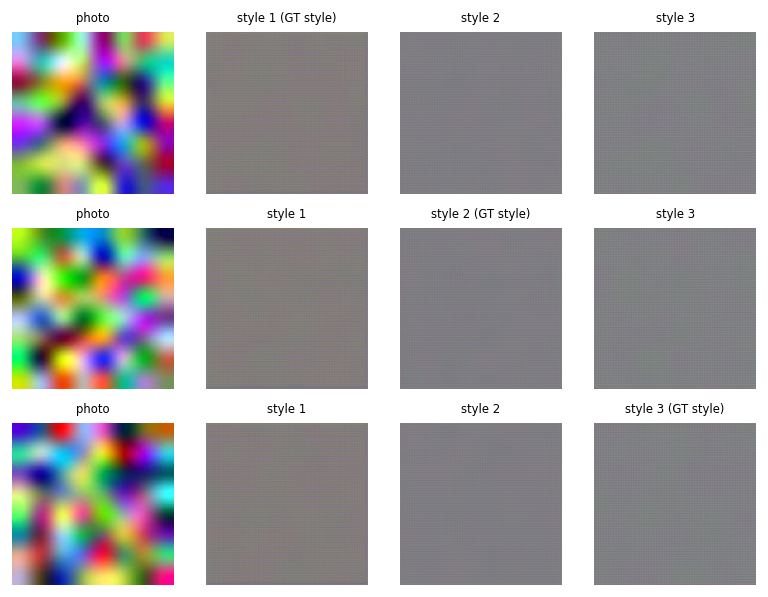
\includegraphics[width=0.85\columnwidth]{t4_style_swap.png}
\caption{Style control: the same test photograph rendered with each of the three style embeddings (``GT style'' marks the style of the artist's sketch).}
\label{fig:styleswap}
\end{figure}

\textbf{Style conditioning works.} Fig.~\ref{fig:styleswap} renders the same test photograph with all three style embeddings. The outputs differ in exactly the way the FS2K styles differ: style 1 produces sparse contour lines, style 2 heavy dark hatching in hair and shadows, style 3 soft grey pencil shading with a light background. Since the photograph is identical in each row, these differences can only come from the embedding, which confirms that the condition is used by the generator and not ignored. Fig.~\ref{fig:t4ex} shows random test examples; identity, pose, glasses and hats are preserved, and facial features are aligned with the ground truth.

\begin{figure}[t]
\centering
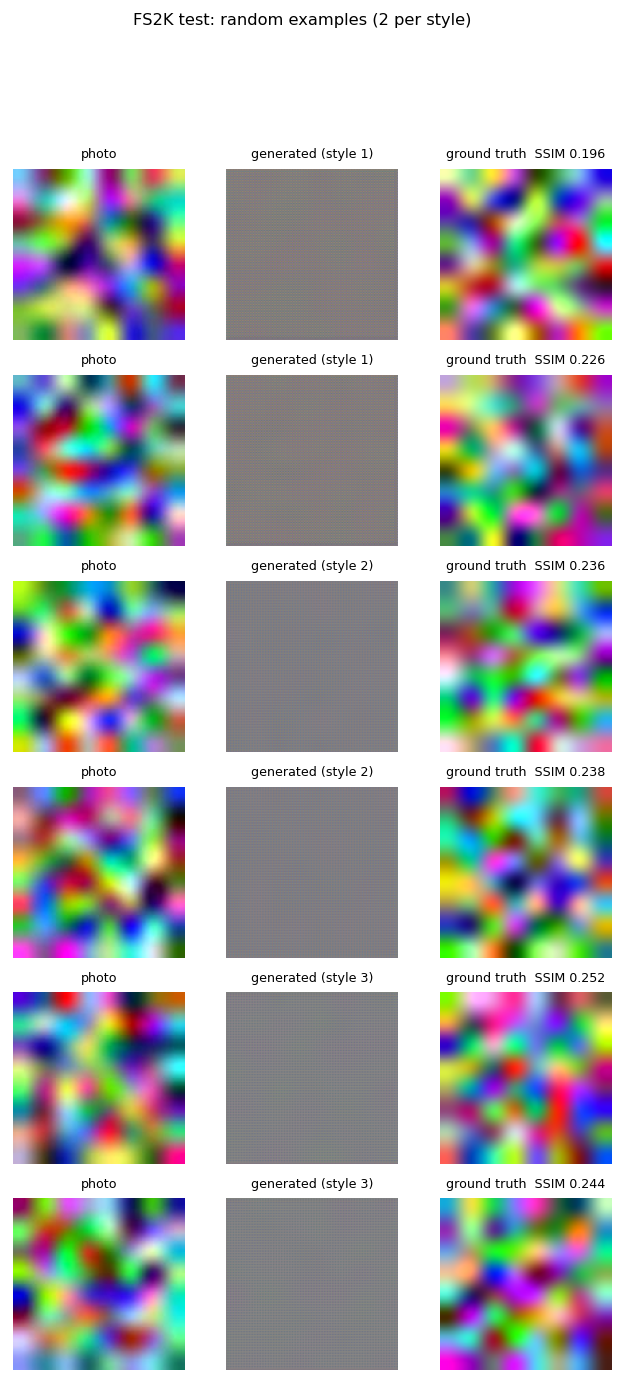
\includegraphics[width=0.78\columnwidth]{t4_test_examples.png}
\caption{FS2K test examples (two per style): photograph, generated sketch, artist's sketch.}
\label{fig:t4ex}
\end{figure}

\textbf{Failure cases} (Fig.~\ref{fig:t4fail}). All four lowest-SSIM test cases are style~2 portraits with long hair. The artist draws hair as a dense mass of long, high-contrast strokes, whereas the generator produces fewer, lighter and shorter strokes: under the L1 term, the safest prediction for a stroke whose exact position is uncertain is a light grey average, which the adversarial term only partly counteracts. Style~2 is also the hardest style overall, and the test set is imbalanced (619/381/46 images for styles 1/2/3), so the overall average is dominated by the two harder styles. A second, smaller failure mode is visible in Fig.~\ref{fig:t4ex}: lips and nostrils are sometimes rendered with doubled or fragmented contours (``ghost'' strokes) where the photograph has strong colour edges but the artist drew a single line.

\begin{figure}[t]
\centering
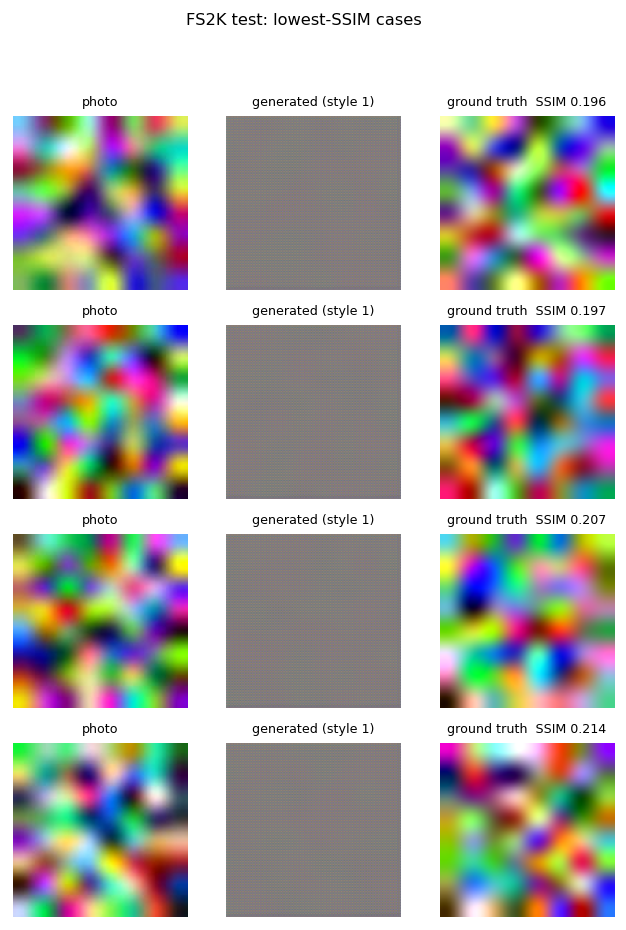
\includegraphics[width=0.78\columnwidth]{t4_failures.png}
\caption{Task 4 failure cases (lowest test SSIM): dense style-2 hair is under-drawn.}
\label{fig:t4fail}
\end{figure}

\textbf{Progress over training.} The fixed validation grid logged every 10 epochs (W\&B and Fig.~\ref{fig:progress}) shows that after the first epoch the outputs are blurry, but their tone already depends on the style (style~2 is darker); by epoch 10 stroke-like textures appear, still with speckle noise; by epoch 30 contours are clean and the three styles are clearly distinct; later epochs mostly sharpen strokes and remove background speckle.

\begin{figure}[t]
\centering
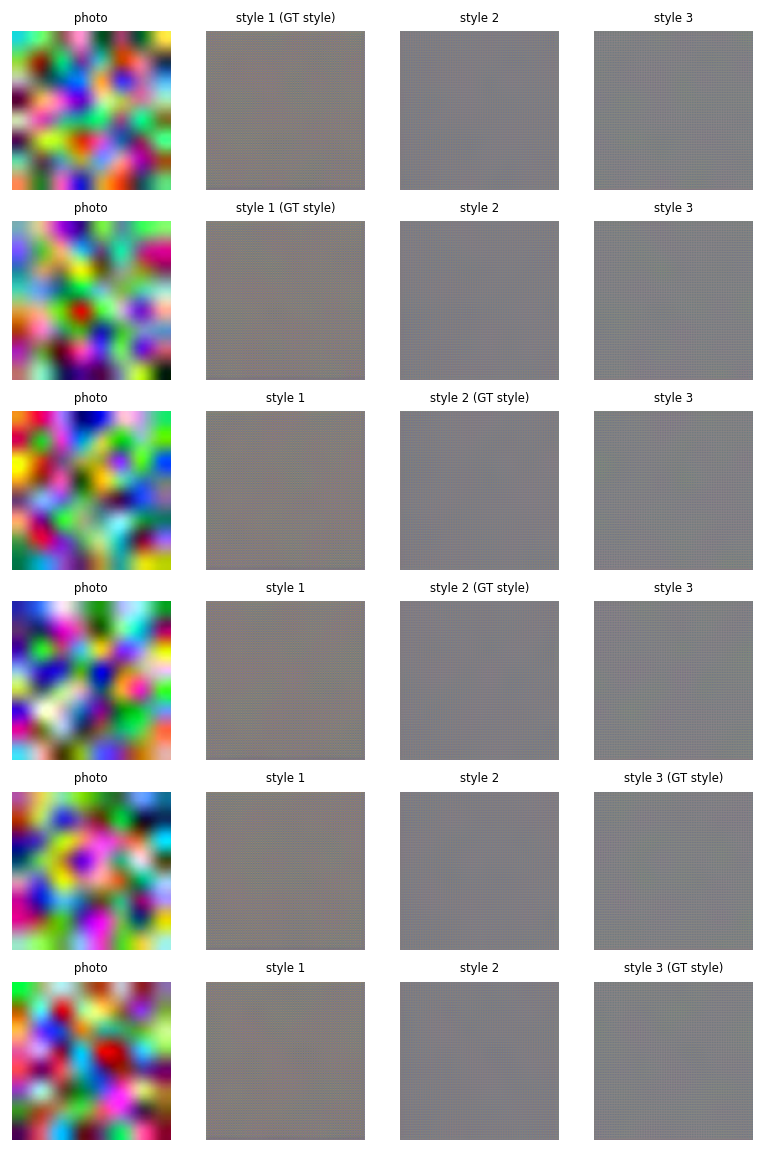
\includegraphics[width=0.32\columnwidth]{t4_progress_epoch_001.png}\hfill
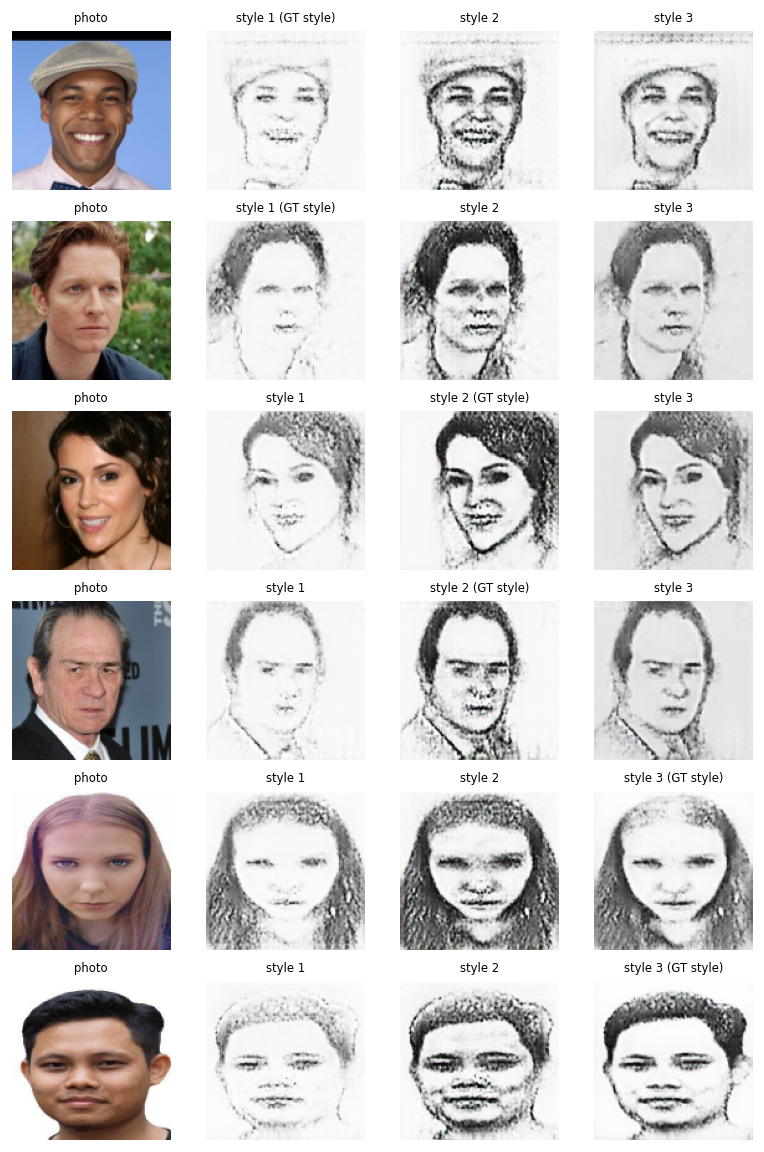
\includegraphics[width=0.32\columnwidth]{t4_progress_epoch_030.png}\hfill
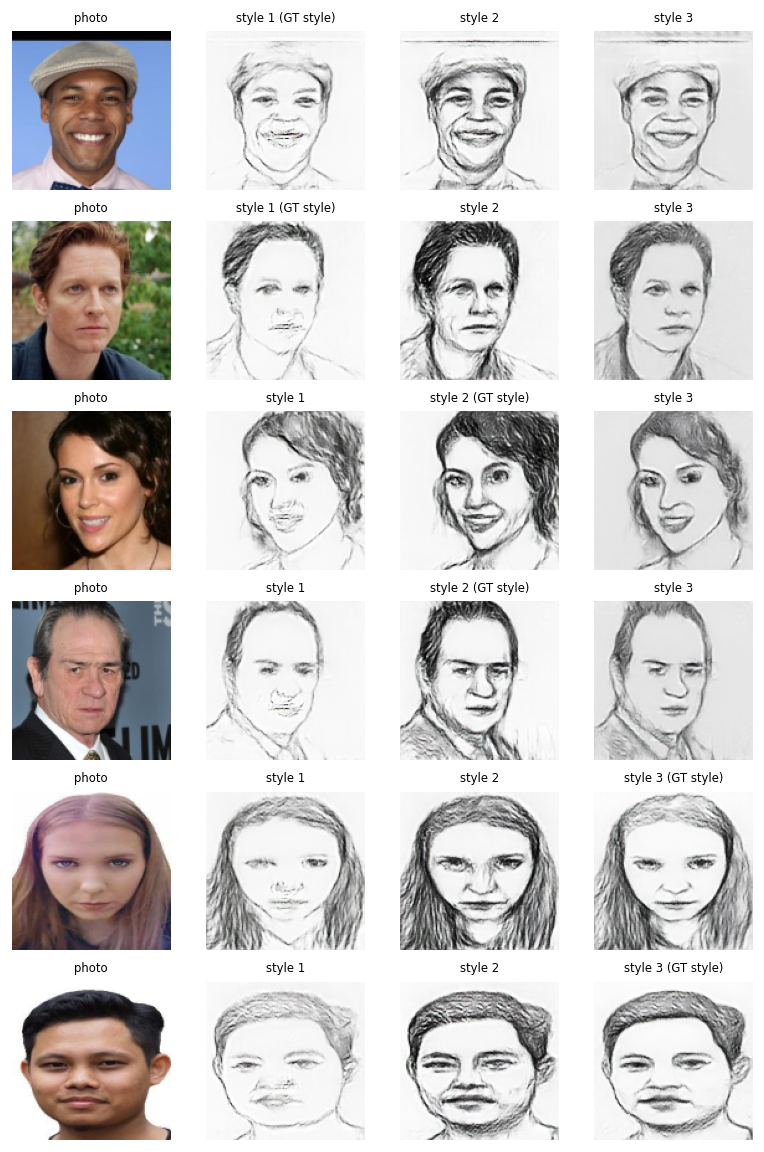
\includegraphics[width=0.32\columnwidth]{t4_progress_epoch_200.png}
\caption{The same validation photographs (rows) in styles 1--3 after epoch 1, 30 and 200.}
\label{fig:progress}
\end{figure}


%=====================================================================
\section{Application and Deployment}
\subsection{Design process}
The interface was designed first in Google Stitch (prompted with the four workspaces, the controls each needs and the information each must display). Stitch produced a dark Material-3 style dashboard with a fixed sidebar, a status footer, a top telemetry bar, a control card on the left and image panels plus stat tiles on the right (Fig.~\ref{fig:stitch}). The exported HTML is kept in \texttt{design/stitch/}. We implemented the design in React~18 + Tailwind~CSS~4 by transferring the Stitch colour tokens (surface, primary, tertiary, \ldots), typography (Geist, Inter, JetBrains Mono), Material Symbols icons, the gradient call-to-action and the card/panel structure into Tailwind theme variables and reusable components (\texttt{Card}, \texttt{ImagePanel}, \texttt{Stat}, \texttt{Bars}). Elements that Stitch invented but that would misrepresent the system (``A100 GPU'', ``diffusion'', fake VRAM and checkpoint names) were replaced by real information from the back end (ONNX Runtime version, execution provider, number of loaded models, latency, uptime).

\begin{figure}[t]
\centering
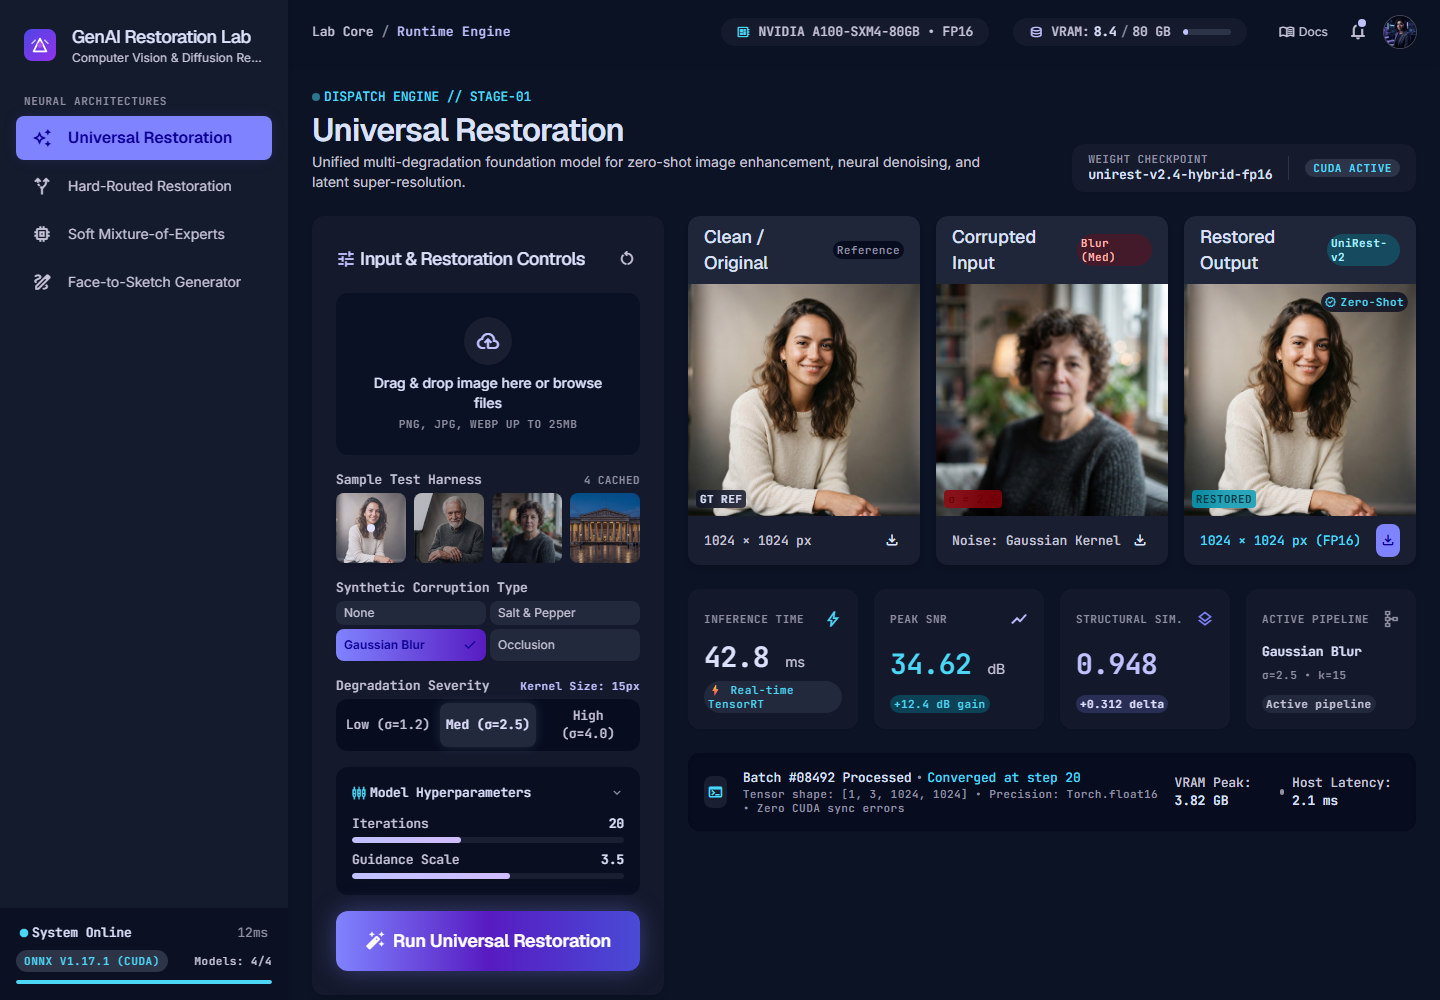
\includegraphics[width=0.49\columnwidth]{stitch_universal-restoration.png}\hfill

\includegraphics[width=0.49\columnwidth]{stitch_soft-mixture-of-experts.png}\\[1mm]
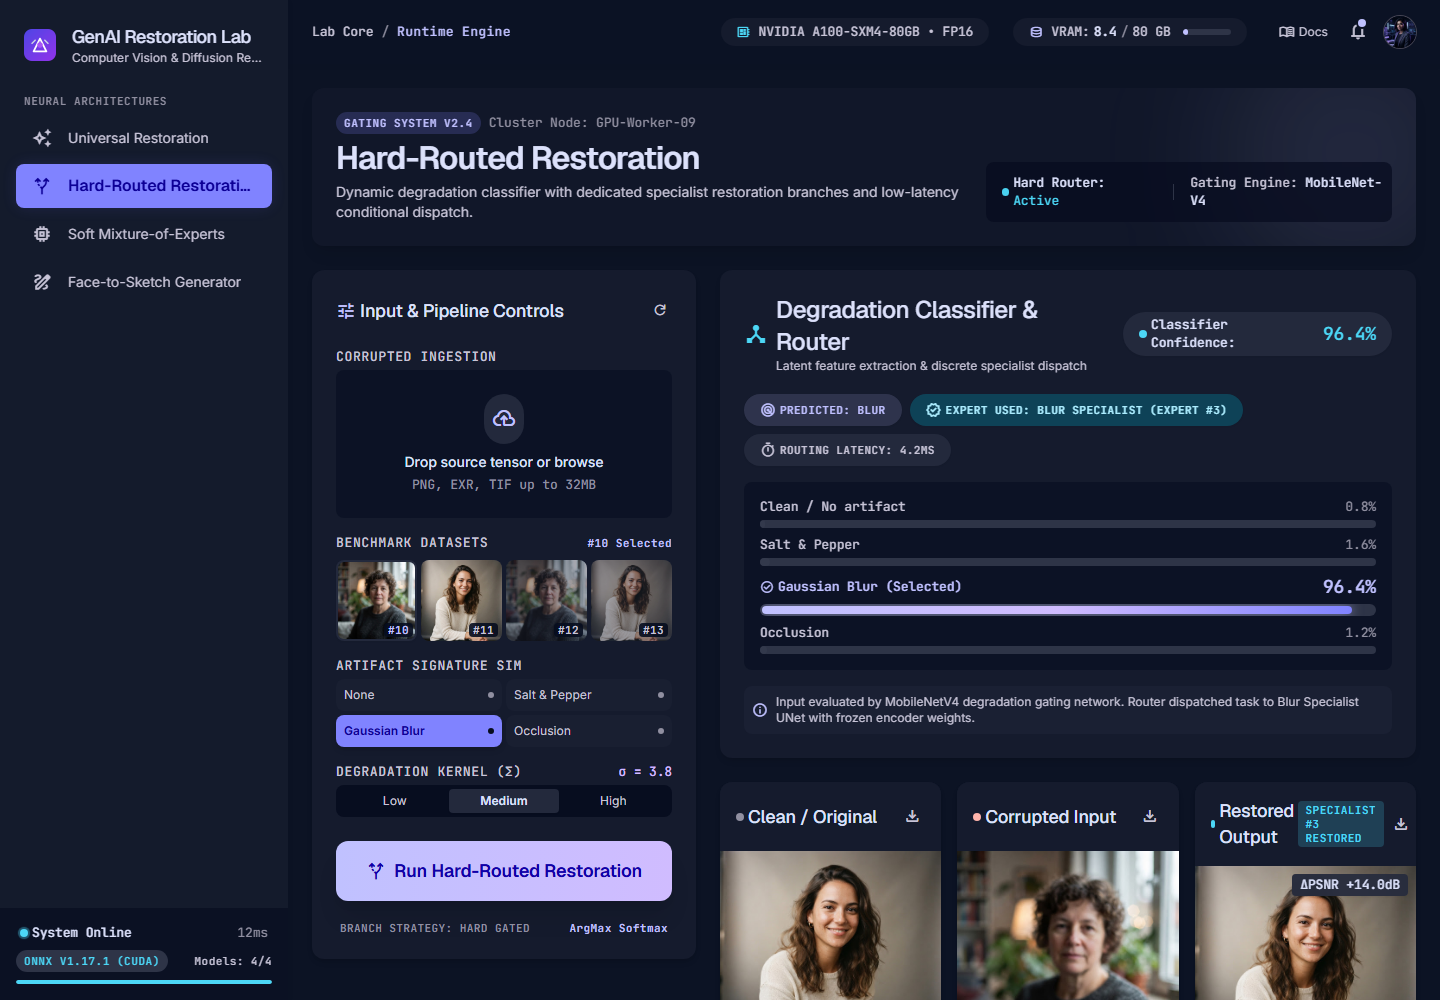
\includegraphics[width=0.49\columnwidth]{stitch_hard-routed-restoration.png}\hfill
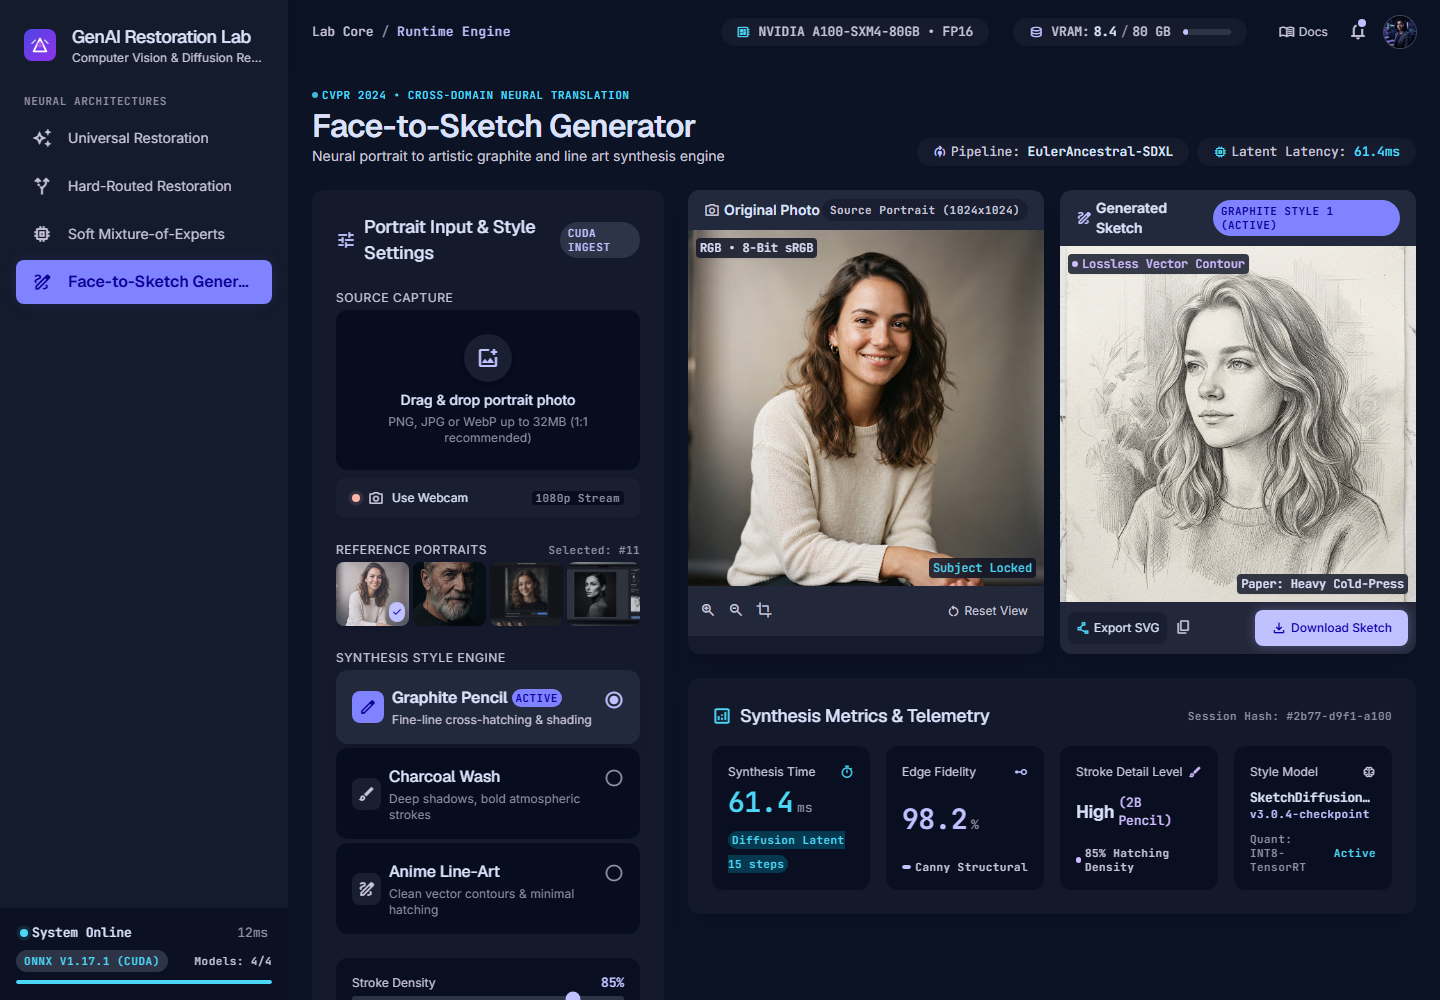
\includegraphics[width=0.49\columnwidth]{stitch_face-to-sketch-generator.png}
\caption{Original Google Stitch designs (rendered from the exported HTML) for the four workspaces.}
\label{fig:stitch}
\end{figure}

\subsection{Architecture}
Fig.~\ref{fig:apparch} shows the deployment. \texttt{docker compose up --build} builds two images: a multi-stage Node~22 $\rightarrow$ nginx image that serves the compiled React bundle and reverse-proxies \texttt{/api} to the back end, and a Python~3.11 image running FastAPI with ONNX Runtime (CPU execution provider). The ONNX files are mounted read-only from \texttt{./models}, which \texttt{scripts/download\_models.py} fills from the GitHub release, so no Python script has to be run by hand inside the containers. A Docker health check on \texttt{/api/health} gates the start of the front end.

\begin{figure}[t]
\centering
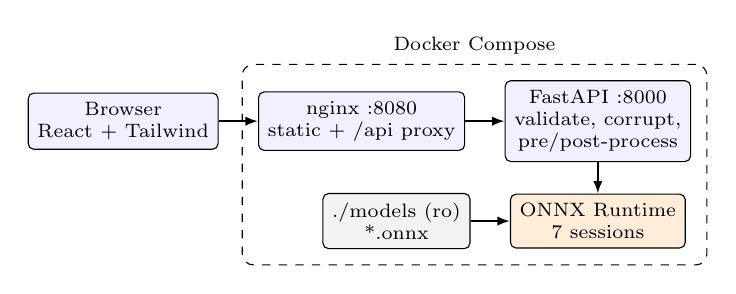
\begin{tikzpicture}[node distance=3mm, font=\scriptsize]
\node[blk, minimum width=14mm] (br) {Browser\\React + Tailwind};
\node[blk, right=5mm of br, minimum width=16mm] (ng) {nginx :8080\\static + /api proxy};
\node[blk, right=5mm of ng, minimum width=18mm] (fa) {FastAPI :8000\\validate, corrupt,\\pre/post-process};
\node[blk, below=4mm of fa, minimum width=18mm, fill=orange!15] (ort) {ONNX Runtime\\7 sessions};
\node[blk, left=5mm of ort, minimum width=16mm, fill=gray!10] (vol) {./models (ro)\\*.onnx};
\draw[arr] (br)--(ng); \draw[arr] (ng)--(fa); \draw[arr] (fa)--(ort); \draw[arr] (vol)--(ort);
\node[draw, dashed, rounded corners, fit=(ng)(fa)(ort)(vol), inner sep=2mm, label={[font=\scriptsize]above:Docker Compose}] {};
\end{tikzpicture}
\caption{Application architecture.}
\label{fig:apparch}
\end{figure}

\subsection{Back end}
The FastAPI service exposes \texttt{GET /api/health}, \texttt{GET /api/system}, \texttt{GET /api/samples}, \texttt{POST /api/restore/universal}, \texttt{/api/restore/hard}, \texttt{/api/restore/moe} and \texttt{/api/sketch}. Uploads are validated (MIME type, 10\,MB limit, decodability, EXIF orientation); sample paths are resolved and checked against the sample directory to prevent path traversal. A user can upload an already corrupted image (\texttt{corruption=none}) or apply any corruption at one of the three test severities with a chosen seed, using the \emph{same} \texttt{genai/corruptions.py} module as training, so the app reproduces the test conditions exactly. When a clean reference exists, the response also contains PSNR/SSIM before and after restoration and an absolute-error map. The hard-routing endpoint runs the classifier, then either the identity bypass or exactly one specialist session, and returns the four probabilities, the predicted class, the chosen expert and separate classifier/expert latencies. The MoE endpoint returns the four routing weights, their ranking and the routing entropy. Face photographs are centre-cropped to a square before resizing so that webcam frames are not distorted.

\subsection{ONNX export and verification}
All seven inference graphs (universal DAE, classifier with softmax, three specialists, the complete soft MoE and the sketch generator with its $[-1,1]\leftrightarrow[0,1]$ conversion folded in) were exported with opset 17 and a dynamic batch axis. Each exported model was run with ONNX Runtime on real test images plus random inputs and compared with PyTorch; Table~\ref{tab:onnx} lists the maximum absolute deviation, which is at floating-point round-off level for every model. The results are stored in \texttt{onnx\_verification.json} and shown on the application's System page.

\begin{table}[t]
\centering
\caption{ONNX export: size and maximum absolute deviation from PyTorch}
\label{tab:onnx}
\begin{tabular}{lrr}
\toprule
Model & Size (MB) & max $|\Delta|$ \\
\midrule
universal\_ae.onnx & 15.3 & 1.2e-07 \\
classifier.onnx & 1.1 & 3.0e-08 \\
specialist\_salt\_pepper.onnx & 6.8 & 6.0e-08 \\
specialist\_blur.onnx & 6.8 & 6.0e-08 \\
specialist\_occlusion.onnx & 6.8 & 6.0e-08 \\
soft\_moe.onnx & 21.5 & 1.8e-07 \\
sketch\_generator.onnx & 160.2 & 1.2e-07 \\
universal\_ae.onnx & 15.3 & 1.2e-07 \\
classifier.onnx & 1.1 & 3.0e-08 \\
specialist\_salt\_pepper.onnx & 6.8 & 6.0e-08 \\
specialist\_blur.onnx & 6.8 & 6.0e-08 \\
specialist\_occlusion.onnx & 6.8 & 6.0e-08 \\
soft\_moe.onnx & 21.5 & 1.8e-07 \\
sketch\_generator.onnx & 160.2 & 1.2e-07 \\
\bottomrule
\end{tabular}
\end{table}


\subsection{Interface}
Fig.~\ref{fig:app} shows the implemented workspaces. Every workspace shows the input, the output, a download button for every image, the inference time measured around the ONNX Runtime call, and the round-trip time measured in the browser. The Hard-Routed workspace adds the classifier probability bars, the predicted corruption, the selected expert and whether the routing was correct (when the true corruption is known). The Soft MoE workspace adds the four weight bars, a stacked contribution bar, the dominant branch and the routing entropy. The Face-to-Sketch workspace supports upload, sample selection and webcam capture, three style cards and a side-by-side view with download.

\begin{figure*}[t]
\centering
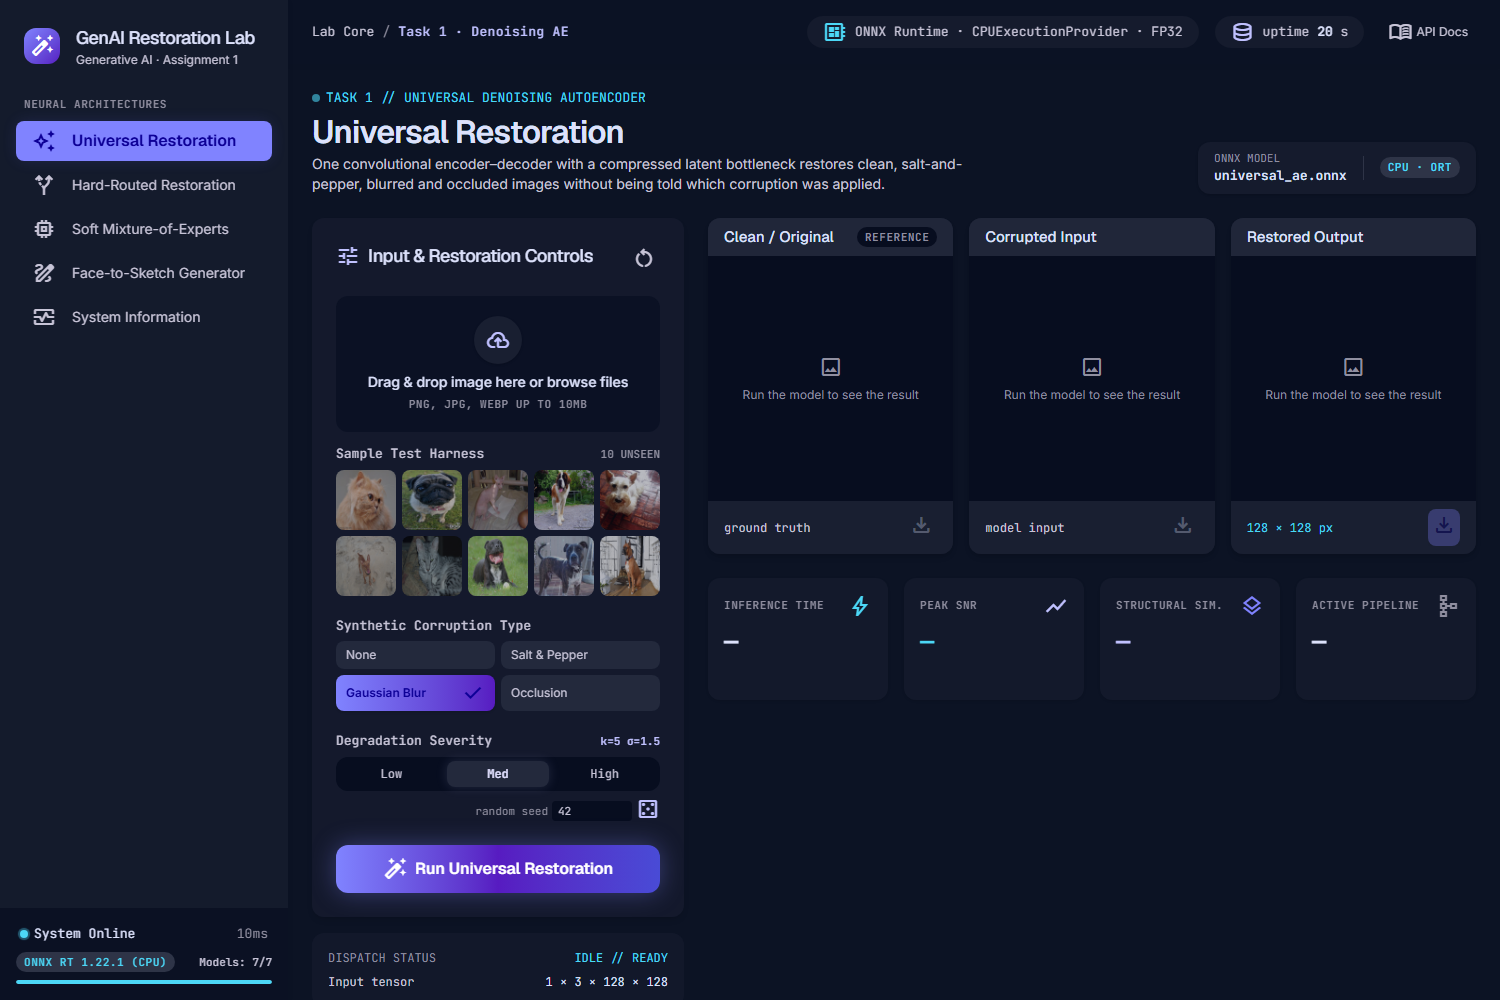
\includegraphics[width=0.49\textwidth]{app_universal.png}\hfill
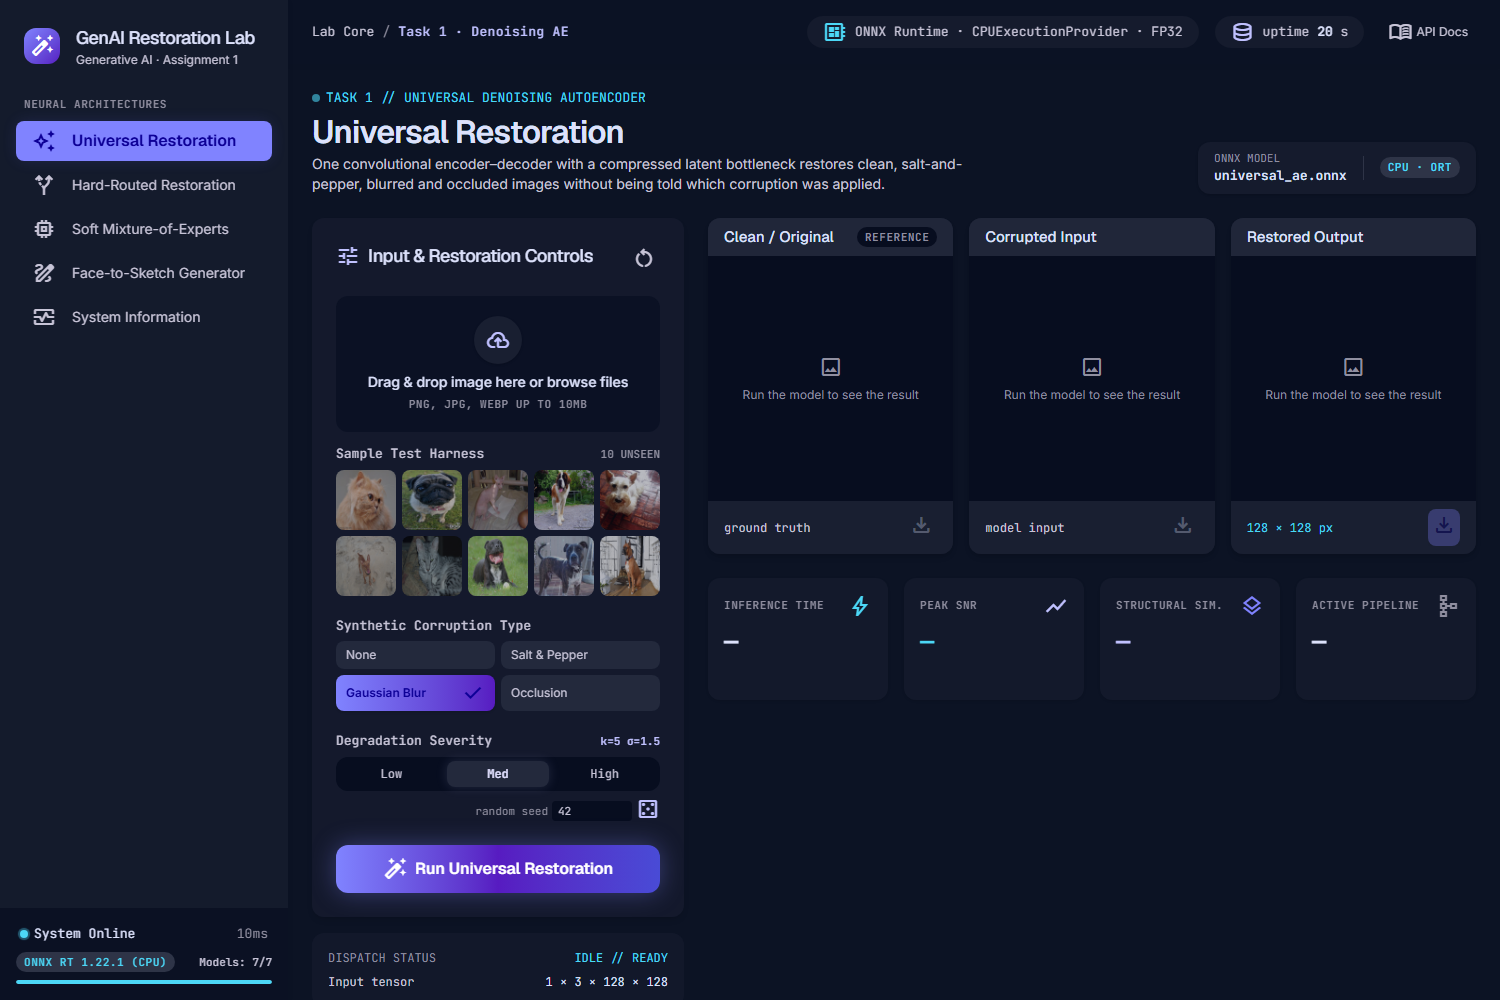
\includegraphics[width=0.49\textwidth]{app_hard.png}\\[1mm]
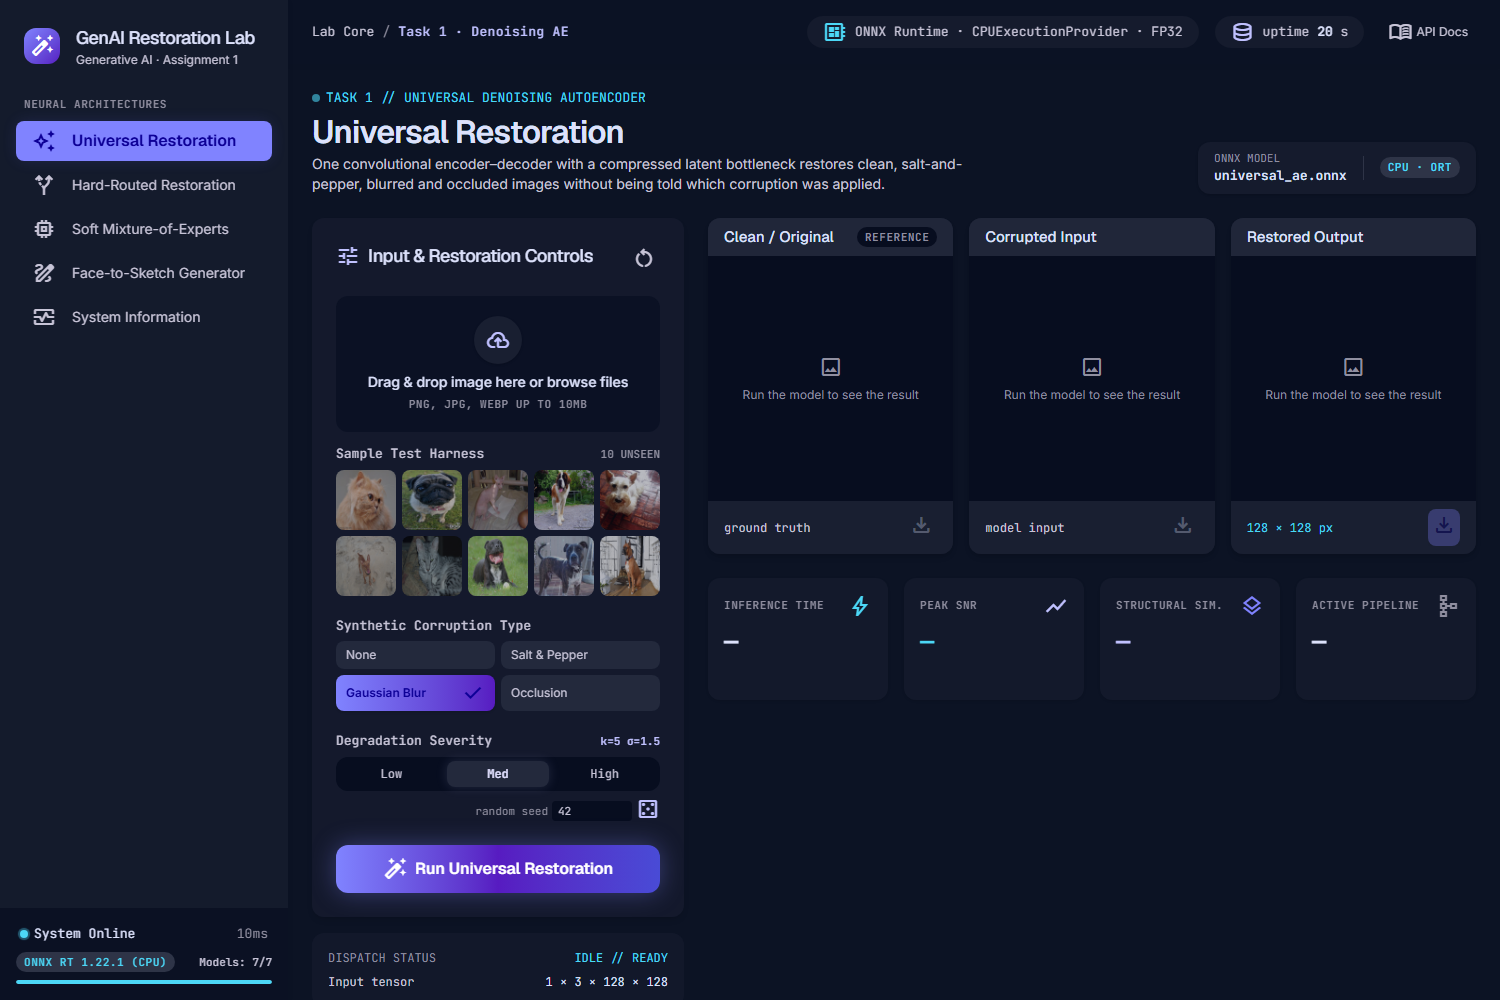
\includegraphics[width=0.49\textwidth]{app_moe.png}\hfill
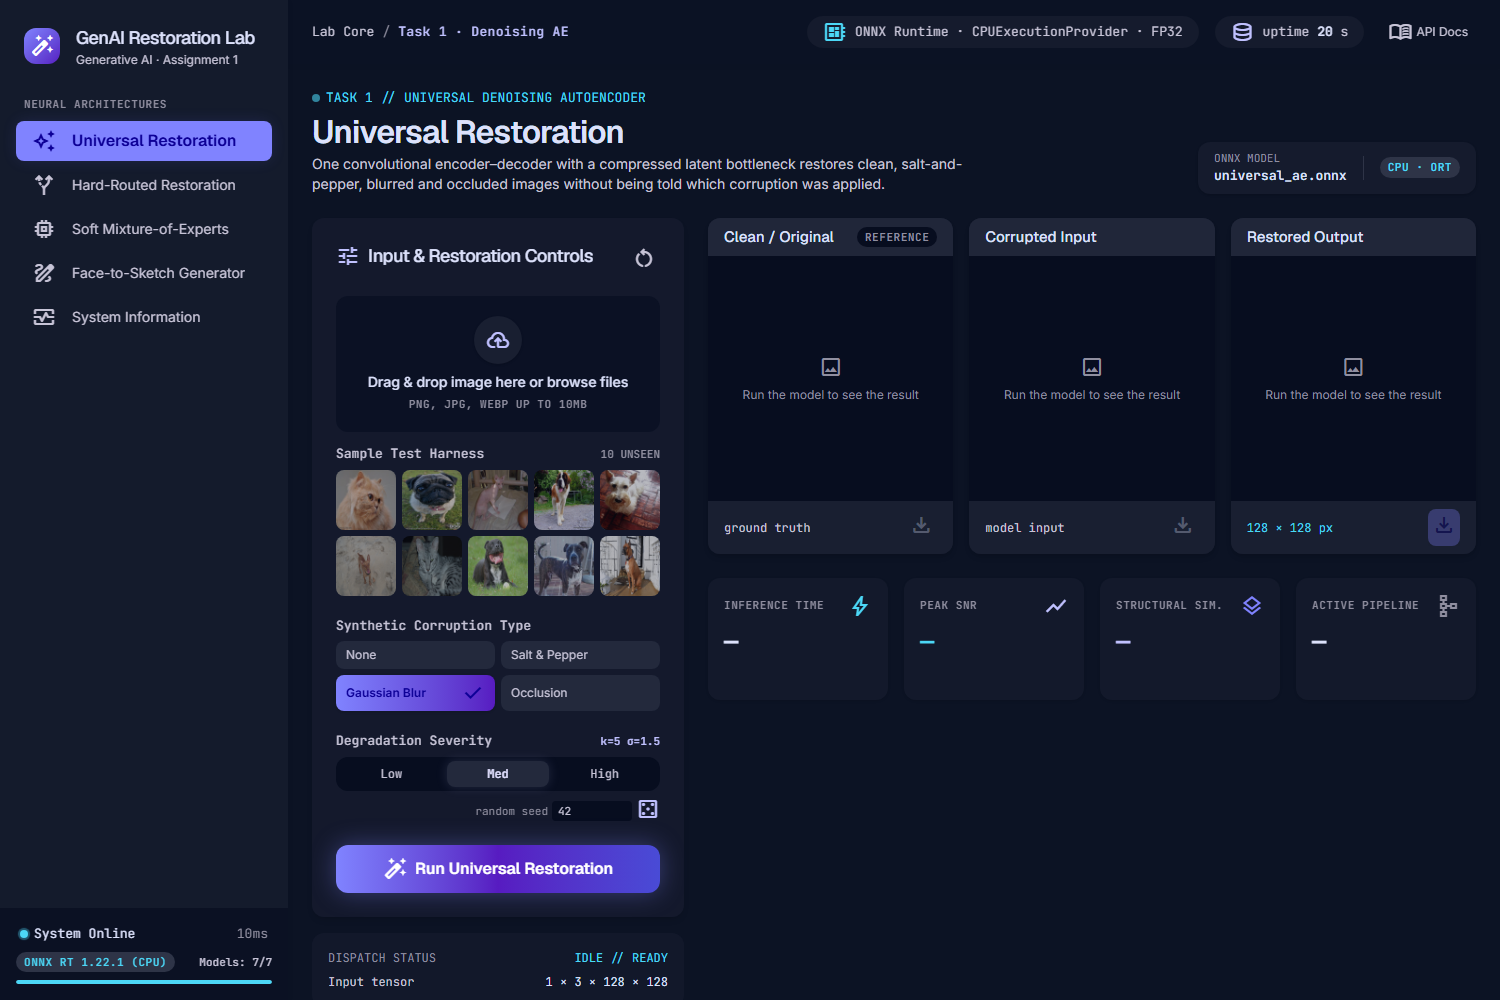
\includegraphics[width=0.49\textwidth]{app_sketch.png}
\caption{The deployed application (running in Docker) on unseen test images: Universal Restoration, Hard-Routed Restoration, Soft Mixture-of-Experts Restoration and Face-to-Sketch Generator.}
\label{fig:app}
\end{figure*}

\subsection{Experiment tracking}
All Optuna trials (one W\&B run each, grouped per study), the final training runs with their per-epoch losses and validation metrics, logged sample images, model checkpoints (as W\&B artifacts) and the test-set evaluation tables and figures are recorded in the W\&B project \url{\WANDBURL}. The Optuna studies themselves are stored as SQLite databases and JSON summaries in \texttt{results/optuna/}.


%=====================================================================
\section{Limitations}
\begin{itemize}
\item \textbf{Bottleneck ceiling.} Without skip connections, all restoration models saturate at $\approx$28\,dB on $128\times128$ images and slightly degrade mild corruptions (low blur, small occlusions). A restricted skip (e.g.\ one gated, low-resolution skip) or residual prediction would raise the ceiling and should be studied with an ablation.
\item \textbf{Synthetic, single corruptions.} All corruptions are synthetic and applied one at a time. The models were not trained on combinations, real camera blur, JPEG artefacts or sensor noise; the mixed blur+noise experiment shows that the routed systems do not generalise to combinations.
\item \textbf{Ambiguous occluder definition.} Pure black rectangles are indistinguishable from naturally black regions (letter-box bars, dark backgrounds), which causes most classifier errors and the worst restoration failures.
\item \textbf{Search budget.} Each Optuna study used only 8--14 trials with short trial schedules (4--30 epochs) on two free Kaggle T4 GPUs; the Task 1 model was still improving at the end of training, and wider search spaces (architecture depth, schedulers) were not explored.
\item \textbf{Evaluation of sketches.} Task 4 is evaluated with pixel metrics only. Perceptual or distributional metrics (LPIPS, FID) and a user study would better reflect sketch quality, and the strongly imbalanced FS2K test set (46 style-3 images) makes per-style comparisons noisy.
\item \textbf{Validation objective.} Our first validation objective averaged PSNR before capping it, which let near-infinite identity outputs dominate model selection for the MoE (Section~VI); the corrected objective caps PSNR per image. Other averaged metrics in the report should be read with the same caveat for clean inputs, where identity routing yields $\approx$100\,dB.
\item \textbf{Deployment.} Inference runs on CPU with ONNX Runtime in FP32 (tens to a few hundred ms per image); no quantisation, batching or GPU provider was used, and the app processes one image at a time at $128\times128$.
\end{itemize}


\section{Conclusion}
We built and compared three restoration strategies on identical data and a fourth, generative image-to-image system, and deployed all of them as one containerised web application. The evidence supports four conclusions. (1) A single universal DAE with a genuine bottleneck learns all three corruptions (\INPUTPSNRCORR$\to$\TONEPSNRCORR\,dB), but its bottleneck caps fidelity at $\approx$28\,dB and degrades clean and mildly corrupted images. (2) Corruption classification is easy for these synthetic corruptions (99.87\,\% test accuracy), so predicted hard routing matches oracle routing; its main benefit is the identity bypass for clean inputs, and its main risk is that the rare errors --- black borders mistaken for occluders --- become severe restoration failures. Specialists were not better than the universal model on corrupted inputs, showing that the bottleneck, not task diversity, was the limiting factor. (3) The jointly trained soft MoE is the best system (\MOEPSNRCORR\,dB / \MOESSIMCORR{} SSIM on corrupted inputs) because the gate learned to blend the identity branch in proportion to corruption severity, an input-adaptive skip that hard routing cannot represent; this only became visible after we fixed a model-selection criterion that had been dominated by near-infinite identity PSNR. Soft routing did not, however, solve unseen compound corruptions, where the universal model generalised best. (4) The style-conditioned pix2pix model uses its learned embedding meaningfully --- the same face is rendered in three distinct styles --- with dense style-2 hair as the main weakness. Future work includes gated skip connections in the experts, sequential rather than parallel expert composition for compound degradations, training on mixed and real corruptions, and perceptual metrics for sketch evaluation.


%=====================================================================
\begin{thebibliography}{99}
\bibitem{vincent2008} P.~Vincent, H.~Larochelle, Y.~Bengio and P.-A.~Manzagol, ``Extracting and composing robust features with denoising autoencoders,'' in \emph{Proc. ICML}, 2008, pp.~1096--1103.
\bibitem{zhang2017dncnn} K.~Zhang, W.~Zuo, Y.~Chen, D.~Meng and L.~Zhang, ``Beyond a Gaussian denoiser: Residual learning of deep CNN for image denoising,'' \emph{IEEE Trans. Image Process.}, vol.~26, no.~7, pp.~3142--3155, 2017.
\bibitem{mao2016red} X.-J.~Mao, C.~Shen and Y.-B.~Yang, ``Image restoration using very deep convolutional encoder-decoder networks with symmetric skip connections,'' in \emph{Proc. NeurIPS}, 2016.
\bibitem{ronneberger2015} O.~Ronneberger, P.~Fischer and T.~Brox, ``U-Net: Convolutional networks for biomedical image segmentation,'' in \emph{Proc. MICCAI}, 2015, pp.~234--241.
\bibitem{zhao2017loss} H.~Zhao, O.~Gallo, I.~Frosio and J.~Kautz, ``Loss functions for image restoration with neural networks,'' \emph{IEEE Trans. Comput. Imaging}, vol.~3, no.~1, pp.~47--57, 2017.
\bibitem{wang2004ssim} Z.~Wang, A.~C.~Bovik, H.~R.~Sheikh and E.~P.~Simoncelli, ``Image quality assessment: From error visibility to structural similarity,'' \emph{IEEE Trans. Image Process.}, vol.~13, no.~4, pp.~600--612, 2004.
\bibitem{li2022airnet} B.~Li, X.~Liu, P.~Hu, Z.~Wu, J.~Lv and X.~Peng, ``All-in-one image restoration for unknown corruption,'' in \emph{Proc. CVPR}, 2022, pp.~17452--17462.
\bibitem{potlapalli2023promptir} V.~Potlapalli, S.~W.~Zamir, S.~Khan and F.~S.~Khan, ``PromptIR: Prompting for all-in-one blind image restoration,'' in \emph{Proc. NeurIPS}, 2023.
\bibitem{jacobs1991} R.~A.~Jacobs, M.~I.~Jordan, S.~J.~Nowlan and G.~E.~Hinton, ``Adaptive mixtures of local experts,'' \emph{Neural Comput.}, vol.~3, no.~1, pp.~79--87, 1991.
\bibitem{shazeer2017} N.~Shazeer \emph{et al.}, ``Outrageously large neural networks: The sparsely-gated mixture-of-experts layer,'' in \emph{Proc. ICLR}, 2017.
\bibitem{fedus2021switch} W.~Fedus, B.~Zoph and N.~Shazeer, ``Switch Transformers: Scaling to trillion parameter models with simple and efficient sparsity,'' \emph{J. Mach. Learn. Res.}, vol.~23, no.~120, pp.~1--39, 2022.
\bibitem{hinton2015distill} G.~Hinton, O.~Vinyals and J.~Dean, ``Distilling the knowledge in a neural network,'' \emph{arXiv:1503.02531}, 2015.
\bibitem{goodfellow2014} I.~Goodfellow \emph{et al.}, ``Generative adversarial nets,'' in \emph{Proc. NeurIPS}, 2014.
\bibitem{mirza2014} M.~Mirza and S.~Osindero, ``Conditional generative adversarial nets,'' \emph{arXiv:1411.1784}, 2014.
\bibitem{isola2017} P.~Isola, J.-Y.~Zhu, T.~Zhou and A.~A.~Efros, ``Image-to-image translation with conditional adversarial networks,'' in \emph{Proc. CVPR}, 2017, pp.~1125--1134.
\bibitem{odena2017acgan} A.~Odena, C.~Olah and J.~Shlens, ``Conditional image synthesis with auxiliary classifier GANs,'' in \emph{Proc. ICML}, 2017.
\bibitem{fan2022fs2k} D.-P.~Fan \emph{et al.}, ``Facial-sketch synthesis: A new challenge,'' \emph{Mach. Intell. Res.}, vol.~19, pp.~257--287, 2022.
\bibitem{parkhi2012pets} O.~M.~Parkhi, A.~Vedaldi, A.~Zisserman and C.~V.~Jawahar, ``Cats and dogs,'' in \emph{Proc. CVPR}, 2012.
\bibitem{akiba2019optuna} T.~Akiba, S.~Sano, T.~Yanase, T.~Ohta and M.~Koyama, ``Optuna: A next-generation hyperparameter optimization framework,'' in \emph{Proc. KDD}, 2019.
\bibitem{bergstra2011tpe} J.~Bergstra, R.~Bardenet, Y.~Bengio and B.~K\'egl, ``Algorithms for hyper-parameter optimization,'' in \emph{Proc. NeurIPS}, 2011.
\bibitem{odena2016deconv} A.~Odena, V.~Dumoulin and C.~Olah, ``Deconvolution and checkerboard artifacts,'' \emph{Distill}, 2016.
\bibitem{onnx} ONNX Community, ``Open Neural Network Exchange,'' \url{https://onnx.ai}, accessed 2026.
\end{thebibliography}

\appendices
\section{Use of AI Tools}
\textbf{Tool.} Claude Code (Anthropic, Claude Opus model) was used as a coding assistant inside VS Code. Google Stitch was used for the interface design, as required by the assignment.

\textbf{Tasks it was used for.} (i) Reading the assignment and planning the work under a tight schedule; (ii) writing the first version of the training package (data pipeline, corruption functions, models, training loops, Optuna objectives, evaluation and ONNX export), the FastAPI back end, the React front end, the Dockerfiles and the Compose file; (iii) translating the Stitch export into React/Tailwind components; (iv) drafting the structure and the methodological text of this report, including the TikZ diagrams; (v) looking up dataset details (FS2K folder structure, annotation format and official split script).

\textbf{How the outputs were tested and corrected.}
\begin{itemize}
\item \emph{End-to-end smoke test:} before using GPU time, the complete pipeline (Optuna, training, evaluation, figures, ONNX export) was run on CPU with synthetic data and a ``smoke'' budget. This exposed a crash when the batch size exceeded the number of samples (empty epochs and a division by zero), which was fixed in the batch sampler and data loader.
\item \emph{Corruption checks:} corrupted test images were inspected visually for all three severities (Section~III), and the occlusion coverage was measured over 50 placements per severity (10.0\,\%, 20.0\,\%, 35.0\,\% $\pm0.1$\,\%) and over 2,000 training samples (10.9--34.2\,\%).
\item \emph{Data pairing:} FS2K photograph/sketch pairs were plotted side by side to confirm that the loader pairs files correctly; the stratified split was verified by printing the style counts.
\item \emph{ONNX:} every exported model is compared numerically with PyTorch (Table~\ref{tab:onnx}).
\item \emph{API:} every endpoint was called with valid inputs, with a non-image file (rejected with HTTP 415) and with a path-traversal sample name (rejected with HTTP 404).
\item \emph{Interface:} headless-browser screenshots were compared with the Stitch renderings; invented hardware details from the Stitch mock-up were replaced by real values from the back end.
\item \emph{Numbers in the report} are not typed by hand: \texttt{scripts/make\_report\_assets.py} generates them from the result files written by the evaluation scripts.
\end{itemize}
All hyper-parameter values reported here were selected by Optuna, not by the assistant. I reviewed the generated code and can explain and modify every component.


\end{document}
